\documentclass[10pt,a4paper,final]{article}
%
\usepackage[utf8x]{inputenc}
\usepackage{ucs}
\usepackage{subfig}
\usepackage{amsmath}
\usepackage{float}
\usepackage{geometry}
\usepackage{anysize} % Soporte para el comando \marginsize
\usepackage{graphicx}
\usepackage{listings}
\usepackage{amsfonts}
\usepackage{amssymb}
\usepackage[spanish]{babel}
%%%%%%%%%%%%%%%%%%%%%%%%%%%%%%%%%%%%%%%%%%%%%%%%%
%%%%%%%%%%%%%%%%%%%%%%%%%%%%%%%%%%%%%%%%%%%%%%%%%
%%%%%%%%%%%%%%%%%%%%%%%%%%%%%%%%%%%%%%%%%%%%%%%%%
\marginsize{2cm}{2cm}{1.5cm}{1.5cm}
%
\begin{document}
\title{Cálculo de flujo subterráneo generado por bombeo}
\author{Christian N. Pfarher, Juan Pablo Garbarino, Marina Castro\\
\textit{Trabajo práctico final de ``Métodos numéricos y simulación'', II-FICH-UNL.}}
\markboth{Método numérico y simulación: TRABAJO FINAL}{}
\date{\today}
\maketitle
%%%%%%%%%%%%%%%%%%%%%%%%%%%%%%%%%%%%%%%%%%%%%%%%%%%%%%%%%%%%%%%%%%%%%%%%%%%%%%%%%%%%%%%%%%%%%%%%%%
%%%%%%%%%%%%%%%%%%%%%%%%%%%%%%%%%%%%%%%%%%%%%%%%%%%%%%%%%%%%%%%%%%%%%%%%%%%%%%%%%%%%%%%%%%%%%%%%%%
%%%%%%%%%%%%%%%%%%%%%%%%%%%%%%%%%%%%%%%%%%%%%%%%%%%%%%%%%%%%%%%%%%%%%%%%%%%%%%%%%%%%%%%%%%%%%%%%%%
\newpage
\tableofcontents
%%%%%%%%%%%%%%%%%%%%%%%%%%%%%%%%%%%%%%%%%%%%%%%%%%%%%%%%%%%%%%%%%%%%%%%%%%%%%%%%%%%%%%%%%%%%%%%%%%
%%%%%%%%%%%%%%%%%%%%%%%%%%%%%%%%%%%%%%%%%%%%%%%%%%%%%%%%%%%%%%%%%%%%%%%%%%%%%%%%%%%%%%%%%%%%%%%%%%
%%%%%%%%%%%%%%%%%%%%%%%%%%%%%%%%%%%%%%%%%%%%%%%%%%%%%%%%%%%%%%%%%%%%%%%%%%%%%%%%%%%%%%%%%%%%%%%%%%
\newpage
\listoffigures % Índice de figuras
%%%%%%%%%%%%%%%%%%%%%%%%%%%%%%%%%%%%%%%%%%%%%%%%%%%%%%%%%%%%%%%%%%%%%%%%%%%%%%%%%%%%%%%%%%%%%%%%%%
%%%%%%%%%%%%%%%%%%%%%%%%%%%%%%%%%%%%%%%%%%%%%%%%%%%%%%%%%%%%%%%%%%%%%%%%%%%%%%%%%%%%%%%%%%%%%%%%%%
%%%%%%%%%%%%%%%%%%%%%%%%%%%%%%%%%%%%%%%%%%%%%%%%%%%%%%%%%%%%%%%%%%%%%%%%%%%%%%%%%%%%%%%%%%%%%%%%%%
\newpage
\listoftables %tablas
\newpage
%%%%%%%%%%%%%%%%%%%%%%%%%%%%%%%%%%%%%%%%%%%%%%%%%%%%%%%%%%%%%%%%%%%%%%%%%%%%%%%%%%%%%%%%%%%%%%%%%%
%%%%%%%%%%%%%%%%%%%%%%%%%%%%%%%%%%%%%%%%%%%%%%%%%%%%%%%%%%%%%%%%%%%%%%%%%%%%%%%%%%%%%%%%%%%%%%%%%%
%%%%%%%%%%%%%%%%%%%%%%%%%%%%%%%%%%%%%%%%%%%%%%%%%%%%%%%%%%%%%%%%%%%%%%%%%%%%%%%%%%%%%%%%%%%%%%%%%%
\section{Introducción}
El flujo subterráneo de agua es un componente importante de todos los sistemas hidráulicos. Tiene un papel central en el presupuesto de agua para uso doméstico, industrial y en agricultura. La administración del recurso, implica tomar decisiones sobre donde perforar para extraer o inyectar y sobre las estrategias de control. También, implica decisiones sobre la calidad del agua producida, lo que a su vez se relaciona con la disponibilidad del recurso.\\
Las reservas de agua subterránea como las \emph{napas} y los \emph{acuíferos} están formadas por la infiltración natural de agua de lluvia. Proveen el líquido a casas e industrias, a través de perforaciones individuales o de la explotación a gran escala por parte de empresas de servicios públicos.\\
Centraremos la atención en los acuíferos. Un acuífero es una formación geológica subterránea, capaz de almacenar y rendir agua. El acuífero ocupa un dominio constituido por un medio poroso: tierra, arena, basaltos, granitos – usualmente fisurados – que exhiben en común el estar constituidos por una matriz sólida y poros. Las condiciones geológicas e hidrológicas determinan su tipo y funcionamiento.
\subsubsection*{Tipos de acuíferos}
Hay dos tipos de \emph{acuíferos}: 
\begin{itemize}
\item \emph{Confinados: }el agua está atrapada entre las capas impermeables de la roca o entre grietas de la formación rocosa. Dicha agua podría encontrarse almacenada a presión. Si perforamos, el nivel de agua asciende hasta situarse en una determinada posición que coincide con el nivel de saturación del acuífero en el área de recarga.\\
Si la topografía es tal que la boca del pozo está por debajo del nivel del agua, el pozo es
surgente o artesiano; si no es así el nivel del agua ascenderá hasta el nivel correspondiente, pero no será surgente. El agua está sometida a una presión superior a la atmosférica y ocupa totalmente los poros o huecos de la formación geológica, saturándola totalmente. No existe zona no saturada. \\
%
\item \emph{No confinados o libres: } los acuíferos pueden estar cerca de la superficie terrestre, con estratos continuos formados por materiales de alta permeabilidad, que se extienden desde la superficie del terreno hasta la base del acuífero. La recarga de este acuífero, se produce debido a una infiltración vertical, a través de la zona no saturada. La recarga también se puede producir a través de flujo subterráneo lateral o desde estratos inferiores.\\
\end{itemize}
%
El problema que se presenta en el presente trabajo, trata el caso de un \emph{acuífero confinado, homogéneo e isótropo} el cual consta de dos pozos de bombeo de agua que extraen, cada uno, un caudal de agua, por un tiempo determinado.
Un medio \emph{homogéneo} es aquel que tiene las mismas propiedades en todas las posiciones. Esto significa que la porosidad y otros parámetros son similares en cualquier posición dentro de la unidad geológica.\\
En un medio poroso compuesto de esferas del mismo diámetro, agrupadas uniformemente, la geometría de los huecos vacíos es la misma en cualquier dirección. De esta manera, la permeabilidad del medio es la misma en cualquier dirección, y el medio se denomina \emph{isotrópico}.
Para la realización del trabajo se utilizó el software de pre y pos proceso GiD \footnote{http://gid.cimne.upc.es/}. Mediante el mismo, se utilizó el \emph{módulo de pre-proceso} para la carga de los datos del problema, mientras que para la simulación se utilizó Tdyn \footnote{es un entorno tridimensional de análisis fluidodinámico (CFD) y multifísica basado en el método de los elementos finitos estabilizado}(\emph{módulo de post-proceso}).
%%%%%%%%%%%%%%%%%%%%%%%%%%%%%%%%%%%%%%%%%%%%%%%%%%%%%%%%%%%%%%%%%%%%%%%%%%%%%%%%%%%%%%%%%%%%%%%%%%
%%%%%%%%%%%%%%%%%%%%%%%%%%%%%%%%%%%%%%%%%%%%%%%%%%%%%%%%%%%%%%%%%%%%%%%%%%%%%%%%%%%%%%%%%%%%%%%%%%
%%%%%%%%%%%%%%%%%%%%%%%%%%%%%%%%%%%%%%%%%%%%%%%%%%%%%%%%%%%%%%%%%%%%%%%%%%%%%%%%%%%%%%%%%%%%%%%%%%
\section{Objetivos}
El objetivo de este trabajo, es simular el flujo, en un medio poroso (acuífero confinado, homogéneo e isótropo), generado por un par de bombas de extracción de agua en un campo de bombeo para visualizar las lineas de corrientes y equipotenciales generadas. \begin{Large}
VER!!!!***********************************
\end{Large}
%%%%%%%%%%%%%%%%%%%%%%%%%%%%%%%%%%%%%%%%%%%%%%%%%%%%%%%%%%%%%%%%%%%%%%%%%%%%%%%%%%%%%%%%%%%%%%%%%%
%%%%%%%%%%%%%%%%%%%%%%%%%%%%%%%%%%%%%%%%%%%%%%%%%%%%%%%%%%%%%%%%%%%%%%%%%%%%%%%%%%%%%%%%%%%%%%%%%%
%%%%%%%%%%%%%%%%%%%%%%%%%%%%%%%%%%%%%%%%%%%%%%%%%%%%%%%%%%%%%%%%%%%%%%%%%%%%%%%%%%%%%%%%%%%%%%%%%%
\section{Base Teórica}
%%%%%%%%%%%%%%%%%%%%%%%%%%%%%%%%%%%%%%%%%%%%%%%%%%%%%%%%%%%%%%%%%%%%%%%%%%%%%%%%%%%%%%%%%%%%%%%%%%%
\subsection{Modelo matemático}
Para la resolución del problema utilizamos \emph{Tdyn}, el cual está basado en la solución numérica de las ecuaciones de \emph{Navier-Stokes} empleando el \emph{FEM}.
\emph{Tdyn} resuelve las ecuaciones de Navier-Stokes en tres dimensiones para un fluido incompresible o ligeramente compresible de un dominio $\Omega$ dado y un intervalo de tiempo $(0,t):$
\begin{eqnarray}
\rho \left(\frac{\partial u}{\partial t}+\left( u \bullet  \nabla \right)u \right)+ \nabla p - \nabla \bullet(\mu \nabla u) &=& \rho f~ \mbox{ en  }\Omega \times (0,t)\\
\nabla \bullet u&=&0 ~ \mbox{ en  } \Omega \times (0,t)
\end{eqnarray}
donde $u = u(x,t)$ denota el vector velocidad, $p=p(x,t)$ el campo de presiones, $\rho$ la densidad (constante), $\mu$ la viscosidad dinámica del fluido y la $f$ la aceleración volumétrica.\\
Las ecuaciones de arriba necesitan ser combinadas con las siguientes condiciones de borde:
\begin{eqnarray}
u &=& u_c \mbox{ en  } \Gamma_D \times (0,t);\\
p &=& p_c \mbox{ en  } \Gamma_P \times (0,t);\\
n \cdot \sigma \cdot g_1=0 \mbox{, } n \cdot \sigma \cdot g_2=0~ \mbox{, } n \cdot u&=&u_M \mbox{ en  } \Gamma_M \times (0,t);\\
u(x,0)&=&u_0(x) \mbox{ en  } \Omega_D \times \lbrace 0 \rbrace ;\\
p(x,0)&=&p_0(x) \mbox{ en  } \Omega_D \times \lbrace 0 \rbrace ;
\end{eqnarray}
En las ecuaciones de arriba, $\Gamma = \partial \Omega$ denota la frontera del dominio $\Omega$, siendo $n$ el vector normal unitario y $g_1$, $g_2$ los vectores tangentes de la frontera $\partial \Omega$, $u_c$ es el campo de velocidad sobre $\Gamma_D$, $p_c$ la presión sobre $\Gamma_P$, $\sigma$ es el campo de tensiones, $u_M$ el valor de la velocidad normal y $u_0$, $p_0$ los campos de velocidad y presión iniciales. La unión de $\Gamma_D$, $\Gamma_P$ y $\Gamma_M$ debe ser $\Gamma$; la intersección entre ellos es el conjunto vacío, ya que un punto de la frontera puede ser parte de un único tipo de superficie, a menos que forme parte del borde entre dos de ellas.
% TDYN usa las ecuaciones de Navier Stoke para calcular el flujo en medios porosos desde que el flujo esta estático hasta que llega
% a un estado de estabilidad que es el que presenta la ec. de darcy (representación del tiempo final de nuestra modelación)
% Las ecuaciones de Navier Stokes son cuando tenemos flujo puro (no un medio poroso) pero se hace una analogía entre un flujo puro y un % medio poroso cambiando el mu (viscocidad del fluido) de la formular de Navier Stoke por la constante K de permeabilidad, simulando
% de esta forma el medio poroso.
% La capa donde entra el agua, la prseión es mayor que la parte donde sale.... y ese es el delta h de la formula de darcy.. h_4-h_3 y 
% L es 
%
% En la superficie inferior del caño al estar succionando, se produce una baja de presión....
La discretización espacial de las ecuaciones de \emph{Navier - Stokes} es realizada mediante el método de elementos finitos, mientras que para la discretización en el tiempo debe considerarse un algoritmo iterativo tal como el \emph{Método de pasos fraccionarios (Fractional Step Method) de dos pasos (implícito)}.

También hay que aclarar que no se utiliza un modelo te turbulencia (como lo es el de Smagorinsky) ya que se está en presencia de un flujo lento (laminar).
%%%%%%%%%%%%%%%%%%%%%%%%%%%%%%%%%%%%%%%%%%%%%%%%%%%%%%%%%%%%%%%%%%%%%%%%%%%%%%%%%%%%%%%%%%%%%%%%%%
\subsection{Ley de Darcy}
La \emph{Ley de Darcy} expresa que el flujo de agua en un medio poroso, homogéneo e isotrópico es proporcional 
a la conductividad del medio poroso o conductividad hidráulica $K$ y a una fuerza conductora o gradiente hidráulico $i$.
\\
La expresión matemática de la \emph{Ley de Darcy} viene dada por la ecuación (\ref{darcy_formula})
\begin{eqnarray}
Q&=&K \frac{h_3 - h_4}{L} A = K \cdot i \cdot A \label{darcy_formula}
\end{eqnarray}
donde:
\begin{itemize}
	\item[$Q=$] gasto, descarga o caudal en $m^3/s$,
	\item[$L=$] longitud en metros de la muestra, %seria la longitud del dominio nuestro.
	\item[$K=$] una constante, actualmente conocida como coeficiente de permeabilidad de Darcy, variable en función del material de la muestra, en $m/s$,
	\item[$A=$] área de la sección transversal de la muestra, en $m^2$,
	\item[$h_3=$] altura, sobre el plano de referencia que alcanza el agua en un tubo colocado a la entrada de la capa filtrante,
	\item[$h_4=$] altura, sobre el plano de referencia que alcanza el agua en un tubo colocado a la salida de la capa filtrante,
	\item[$i=$] $\frac{h_3 - h_4}{L}=$ el gradiente hidráulico.
\end{itemize}
%
\begin{figure}[tbhp]
\centerline{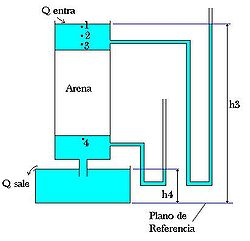
\includegraphics[scale=0.6]{img/darcy_grafica}}
\caption{Ley de Darcy}
\label{graf_leydarcy}
\end{figure}
%
%flujo laminar: es flujo es lento y en el movimiento influyes nas propiedades del seulo por ser lento justamente....
La ley de Darcy es válida para todo suelo donde el flujo sea laminar (esto es, que tiene un movimiento lento): arenas finas a medias, arenas gruesas bien graduadas, arcillas y limos. Entre sus limitaciones, es posible afirmar que la constante de proporcionalidad $K$ no es propia del medio poroso, sino que depende de las características del fluido (peso específico y viscosidad cinemática). 
El factor $K$ se puede descomponer como se puede ver en (\ref{k_descompuesto}) 
\begin{eqnarray}
	K&=& k \cdot x \cdot \gamma \cdot \mu \label{k_descompuesto}
\end{eqnarray}
donde: 
\begin{itemize}
	\item[$K=$] permeabilidad de Darcy o conductividad hidráulica,
	\item[$k=$] permeabilidad intrínseca (depende solo del medio poroso)
	\item[$\gamma=$] peso específico del fluido
	\item[$\mu=$] viscosidad dinámica del fluido
\end{itemize}
Aunque sabemos que $K$ depende tanto del medio como del propio fluido, como la parte que depende del fluido normalmente es despreciable (ya que estamos en presencia de agua, y la viscosidad y peso específico varían muy poco cuando la temperatura varía muy poco), a efectos práctico,s asumimos que la $K$ de Darcy, o \emph{conductividad hidráulica} es una característica del medio poroso.
\\
En algunas circunstancias, la relación entre el caudal y el gradiente hidráulico no es lineal.
Esto puede suceder cuando el valor de $K$ es muy bajo o cuando las velocidades del flujo son muy altas.
En el flujo subterráneo las velocidades son muy lentas y prácticamente siempre la relación es lineal, salvo en las proximidades de captaciones bombeando en ciertas condiciones.
%%%%%%%%%%%%%%%%%%%%%%%%%%%%%%%%%%%%%%%%%%%%%%%%%%%%%%%%%%%%%%%%%%%%%%%%%%%%%%%%%%%%%%%%%%%%%%%%%%
%%%%%%%%%%%%%%%%%%%%%%%%%%%%%%%%%%%%%%%%%%%%%%%%%%%%%%%%%%%%%%%%%%%%%%%%%%%%%%%%%%%%%%%%%%%%%%%%%%
%%%%%%%%%%%%%%%%%%%%%%%%%%%%%%%%%%%%%%%%%%%%%%%%%%%%%%%%%%%%%%%%%%%%%%%%%%%%%%%%%%%%%%%%%%%%%%%%%%
\section{Desarrollo}
%%%%%%%%%%%%%%%%%%%%%%%%%%%%%%%%%%%%%%%%%%%%%%%%%%%%%%%%%%%%%%%%%%%%%%%%%%%%%%%%%%%%%%%%%%%%%%%%%%
Para resolver el problema, se hicieron 2 simulaciones similares pero una con un dominio levemente más pequeño que la otra.
\subsection{Datos del problema}
Los datos para ambas geometrías del problema son los que se presentan a continuación:
\label{datos_problema}
\subsection*{Geometría 1 (de ahora en más la llamaremos \emph{G1}): }
\label{geometria1}
\begin{itemize}
	\item Discretización del área a modelar:	
	\begin{itemize}
		\item Dominio: $x=100 ~\left[m\right]$, $y=100 ~\left[m\right]$
		\item Acuífero confinado, homogéneo e isótropo $(K_{xx} = K_{yy} = K_{zz})$
		\item Espesor del acuífero: $20 ~\left[m\right]$
	\end{itemize}
	%
	\item Coordenadas de ubicación de los Pozos de bombeo:
	\begin{itemize}
		\item Pozo Bombeo 1: $x=17.5~~\left[m\right]$, $y=77.5 ~~\left[m\right]$
		\item Pozo Bombeo 2: $x=65.0~~\left[m\right]$, $y=22.5 ~~\left[m\right]$
	\end{itemize}
	%
	\item Caudal de bombeo:
	\begin{itemize}
		\item Pozo Bombeo 1: $60~\left[\frac{m³}{h}\right]$
		\item Pozo Bombeo 2: $40~\left[\frac{m³}{h}\right]$
	\end{itemize}
	\item Diámetro del pozo: $0.5 [m]$
	\item Profundidad del pozo $15 [m]$
	\item Transmisividad: $600~\left[\frac{m^2}{d}\right]$ \begin{LARGE}
	eso no se si va!!!
	\end{LARGE}\\
\end{itemize}
%
\subsection*{Geometría 2: (de ahora en más la llamaremos \emph{G2}):}
\label{geometria2}
\begin{itemize}
	\item Discretización del área a modelar:	
	\begin{itemize}
		\item Dominio: $x=200 ~\left[m\right]$, $y=200 ~\left[m\right]$
		\item Acuífero confinado, homogéneo e isótropo $(K_{xx} = K_{yy} = K_{zz})$
		\item Espesor del acuífero: $20 ~\left[m\right]$
	\end{itemize}
	%
	\item Coordenadas de ubicación de los Pozos de bombeo:
	\begin{itemize}
		\item Pozo Bombeo 1: $x=30.0 ~~\left[m\right]$, $y=135.0 ~~\left[m\right]$
		\item Pozo Bombeo 2: $x=150.0~~\left[m\right]$, $y=50.0 ~~\left[m\right]$
	\end{itemize}
	%
	\item Caudal de bombeo:
	\begin{itemize}
		\item Pozo Bombeo 1: $60~\left[\frac{m³}{h}\right]$
		\item Pozo Bombeo 2: $40~\left[\frac{m³}{h}\right]$
	\end{itemize}
	\item Diámetro del pozo: $0.5 [m]$
	\item Profundidad del pozo $15 [m]$
	\item Transmisividad: $600~\left[\frac{m^2}{d}\right]$ \begin{LARGE}
	eso no se si va!!!
	\end{LARGE}\\
\end{itemize}
%%%%%%%%%%%%%%%%%%%%%%%%%%%%%%%%%%%%%
\subsubsection{Cálculo de la velocidad de extracción de agua a partir del caudal}
\label{subseccion_transformacion_caudal}
Dado que el caudal de los pozos para ambas geometrías es el mismo, se procedió a convertir las unidades de los datos del problema (Caudal de extracción de los pozos a velocidad) para poder ingresarlas en el software de simulación.
En dinámica de fluidos, \emph{caudal} es la cantidad de fluido que avanza en una unidad de tiempo. Se denomina también ``Caudal volumétrico" o ``Índice de flujo fluido". El cálculo del caudal de agua viene expresado por:
\begin{equation}
Q=V \cdot S
\label{caudal}
\end{equation}
donde en la ecuación (\ref{caudal}) $Q$ es el caudal, $V$ es la velocidad y $S$ es la sección de la tubería
%
\begin{itemize}
\item Pozo de Bombeo 1: a partir de la ec. (\ref{caudal}) y dado que se conoce el caudal del pozo de bombeo 1 $Q_1=60 \left[\frac{m³}{h} \right]$ se puede calcular la velocidad de extracción $V_1$ como:\\
\begin{eqnarray*}
Q_1&=&V_1 \cdot S_1 \\
Q_1/S_1&=&V_1 \\
\frac{60 \left[\frac{m^3}{h}\right]}{\pi \cdot r^2} &=&V_1~~\textrm{donde $r$ es el radio de la tubería}\\
\mbox {dado que $r=0.25 \left[m\right]$ y reemplazando}\\
\frac{1 \left[h\right]}{3600 \left[s\right]}\cdot\frac{60 \left[\frac{m^3}{h}\right]}{\pi \cdot 0.25^2 [m^2]}&=&V_1 \\
0.084883 \left[\frac{m}{s}\right]& = & V_1\\
0.085 \left[\frac{m}{s}\right]&\approx& V_1\\
\end{eqnarray*}
\item Pozo de Bombeo 2: procediendo de la misma manera escrita arriba y con el caudal del pozo de bombeo 2 $Q_2=40 \left[\frac{m³}{h} \right]$ se puede calcular la velocidad de extracción $V_2$ como:\\
\begin{eqnarray*}
Q_2&=&V_2 \cdot S_2 \\
Q_2/S_2&=&V_2 \\
\frac{40 \left[\frac{m^3}{h}\right]}{\pi \cdot r^2} &=&V_1~~\textrm{donde $r$ es el radio de la tubería}\\
\mbox {dado que $r=0.25 \left[m\right]$ y reemplazando}\\
\frac{1 \left[h\right]}{3600 \left[s\right]}\cdot\frac{40 \left[\frac{m^3}{h}\right]}{\pi \cdot 0.25^2 [m^2]}&=&V_2 \\
0.056588 \left[\frac{m}{s}\right]& = & V_2\\
0.057 \left[\frac{m}{s}\right]&\approx& V_2\\
\end{eqnarray*}
\end{itemize}
%%%%%%%%%%%%%%%%%%%%%%%%%%%%%%%%%%%%%%%%%%%%%%%%%%%%%%%%%%%%%%%%%%%%%%%%%%%%%%%%%%%%%%%%%%%%%%%%%%%
\subsection{Definición de Geometría}
Para la geometría en tres dimensiones se tiene los siguientes datos:
En las figuras (\ref{100_xy_cotas}) y (\ref{100_xz_cotas}) se pueden observar
las dimensiones de la \emph{G1} según los datos del problema. Análogamente, pero para \emph{G2}, se presentan las cotas en las figuras (\ref{200_xy_cotas}) y (\ref{200_xz_cotas}).
Hay que aclarar aquí, que en ambas geometrías el cuadrado de $10~m.~x~10~m.$ que se visualiza
alrededor de ambos pozos en las figuras (\ref{100_xy_cotas}), (\ref{100_xz_cotas}), (\ref{200_xy_cotas}) y (\ref{200_xz_cotas}), solo fueron dibujados con el
objetivo, de a posteriori, realizar un refinamiento del dominio en la zona que más interesa visualizar.\\
%
\begin{figure}[tbhp]
\centerline{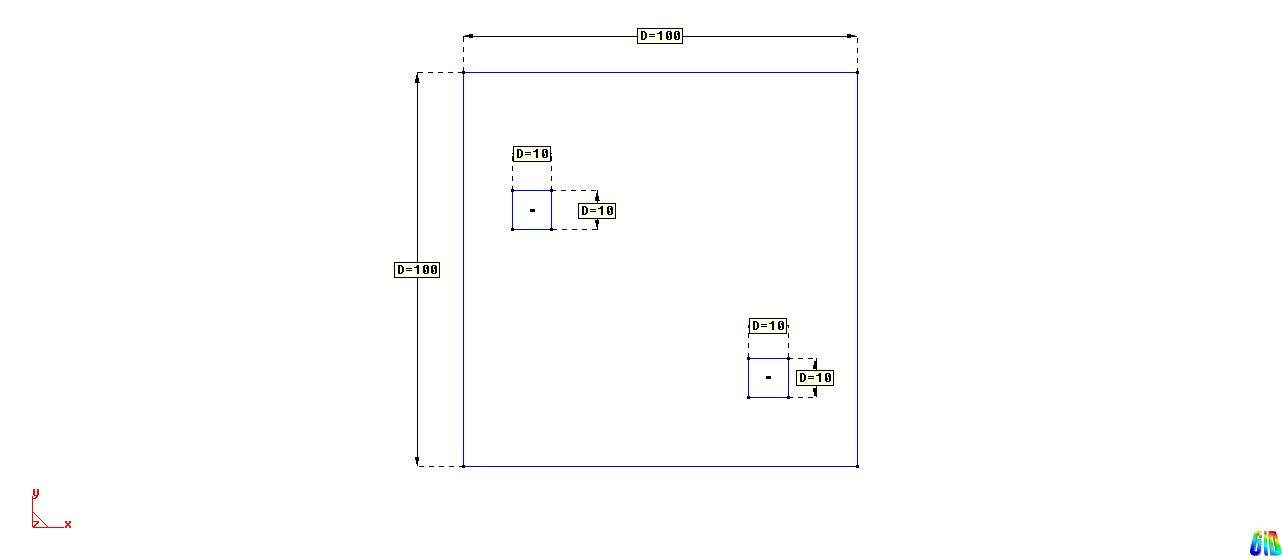
\includegraphics[scale=0.5]{img/100m/100_xy_cotas}}
\caption{Vista de las cotas en el Plano XY para \emph{G1}}
\label{100_xy_cotas}
\end{figure}
%
\begin{figure}[tbhp]
\centerline{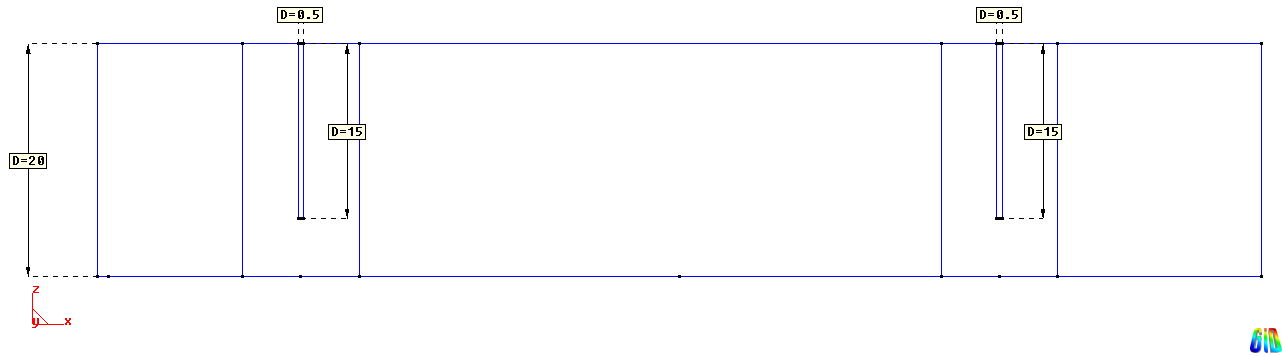
\includegraphics[scale=0.4]{img/100m/100_xz_cotas}}
\caption{Vista de las cotas en el Plano XZ para \emph{G1}}
\label{100_xz_cotas}
\end{figure}
%
%
\begin{figure}[tbhp]
\centerline{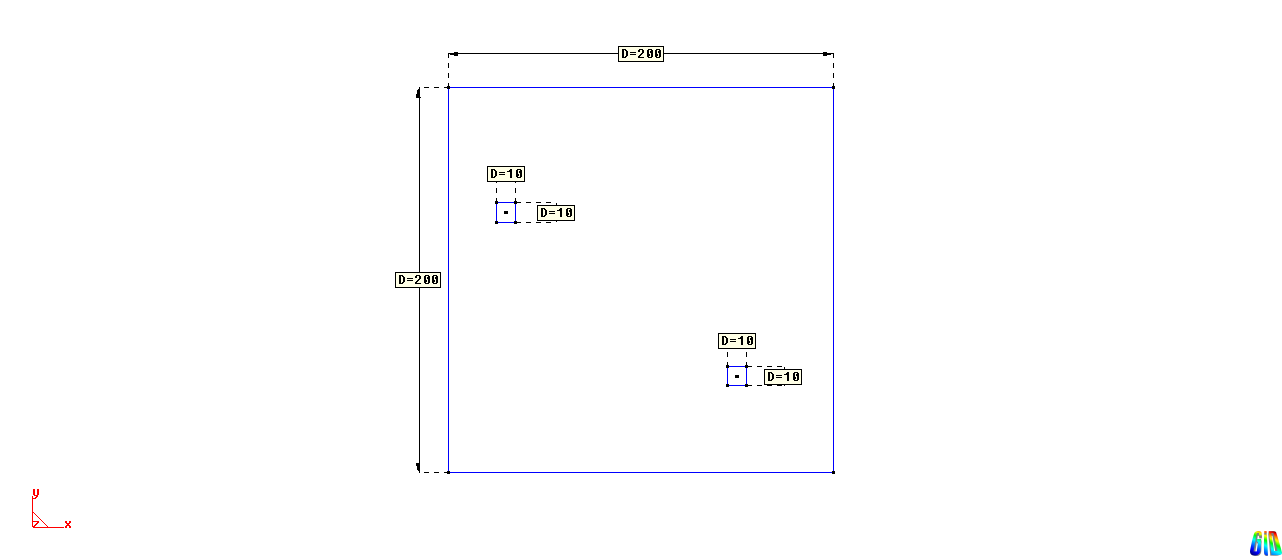
\includegraphics[scale=0.5]{img/200m/200_xy_cotas}}
\caption{Vista de las cotas en el Plano XY para \emph{G2}}
\label{200_xy_cotas}
\end{figure}
%
\begin{figure}[tbhp]
\centerline{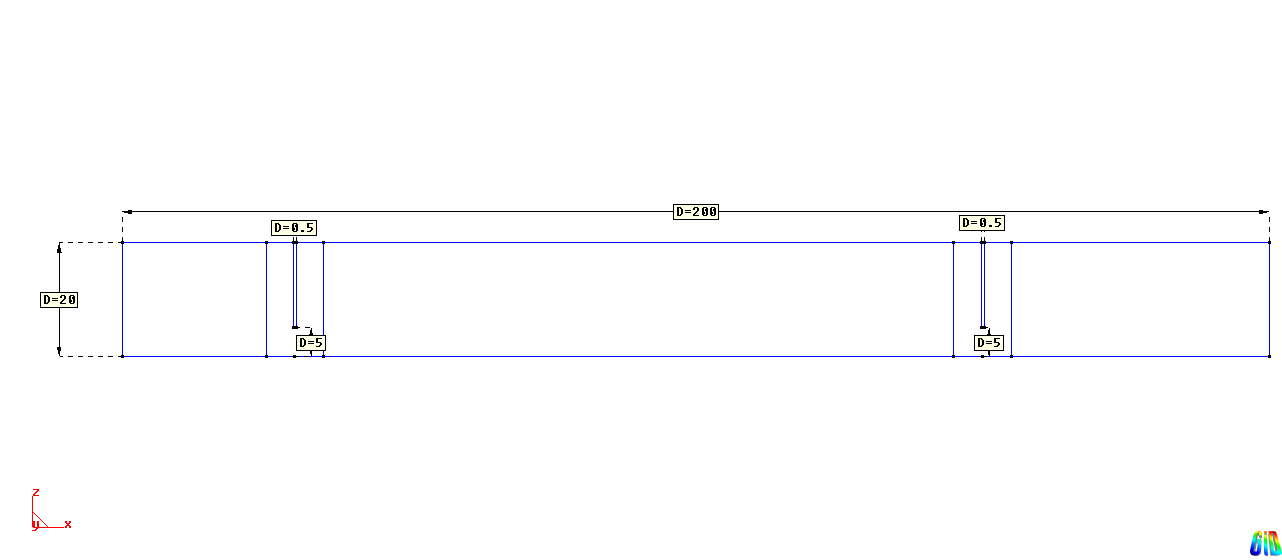
\includegraphics[scale=0.4]{img/200m/200_xz_cotas}}
\caption{Vista de las cotas en el Plano XZ para \emph{G2}}
\label{200_xz_cotas}
\end{figure}
%
En la tabla (\ref{tabla_lista_entidades}) se presentan los datos de los elementos que forman G1 y G2 respectivamente:
%
\begin{table}[tbhp]
\begin{center}\begin{tabular}{ccc}
\hline \textbf{Tipo/Geometría} & \textbf{G1} & \textbf{G2} \\ 
\hline Número de puntos: & 34 & 32 \\ 
\hline Número de líneas: & 48 & 48 \\ 
\hline Número de superficies: & 24 & 24 \\ 
\hline Número de volúmenes: & 3 & 3 \\ 
\hline 
\label{tabla_lista_entidades}
\end{tabular}\end{center}
\caption{Cantidad de puntos, lineas, superficies y volúmenes para \emph{G1} y \emph{G2}}
\end{table}
%
%
%%%%%%%%%%%%%%%%%%%%%%%%%%%%%%%%%%%%%%%%%%%%%%%%%%%%%%%%%%%%%%%%%%%%%%%%%%%%%%%%%%%%%%%%%%%%%%%%%%%
\subsection{Propiedades del medio y de los materiales}
A partir de los datos del problema, se tuvieron que realizar conversiones de unidades y el cálculo de diferentes valores para ser ingresados en el programa \emph{GID} para definir los parámetros del modelo.
Las propiedades asignadas son las mismas para ambas geometrías \emph{G1} y \emph{G2}, por lo cual solo se especificarán una sola vez.
%%%%%%%%%%%%%%%%%%%%%%%%%%%%%%
\subsubsection{Material Suelo}
En la pestaña ransol de la ventana de materiales de fluidos para el material suelo de  se introdujeron los siguientes valores:
\begin{itemize}
\item Modelo de Fluido: flujo incompresible (la densidad del fluido permanece constante con el tiempo $\rho = cte.$)
\item Densidad: $999.7~Kg/m^3$ (agua a $10° C$) \footnote{Datos dados por GID}
\item Viscosidad: $0.001307~Pa.s$ (agua a $10° C$)\footnote{Datos dados por GID}
\item Resistencia de la Ley de Darcy:
\begin{equation}
\begin{pmatrix}{}
0.0000017 & 0.0 & 0.0 \\ 
0.0 & 0.0000017 & 0.0 \\ 
0.0 & 0.0 & 0.0000017
\end{pmatrix} [1/m²]
\label{matrizdarcys}
\end{equation}
Debido a que se está en presencia de un acuífero isótropo (homogéneo en todo el suelo), en (\ref{matrizdarcys}) se puede observar que sólo la diagonal principal de la matriz presenta valores diferentes de cero.
\end{itemize}
En la figura \ref{100_perspectiva_material_agua} se puede observar la asignación del material definido a la parte del dominio correspondiente.
%
\begin{figure}[tbhp]
\centerline{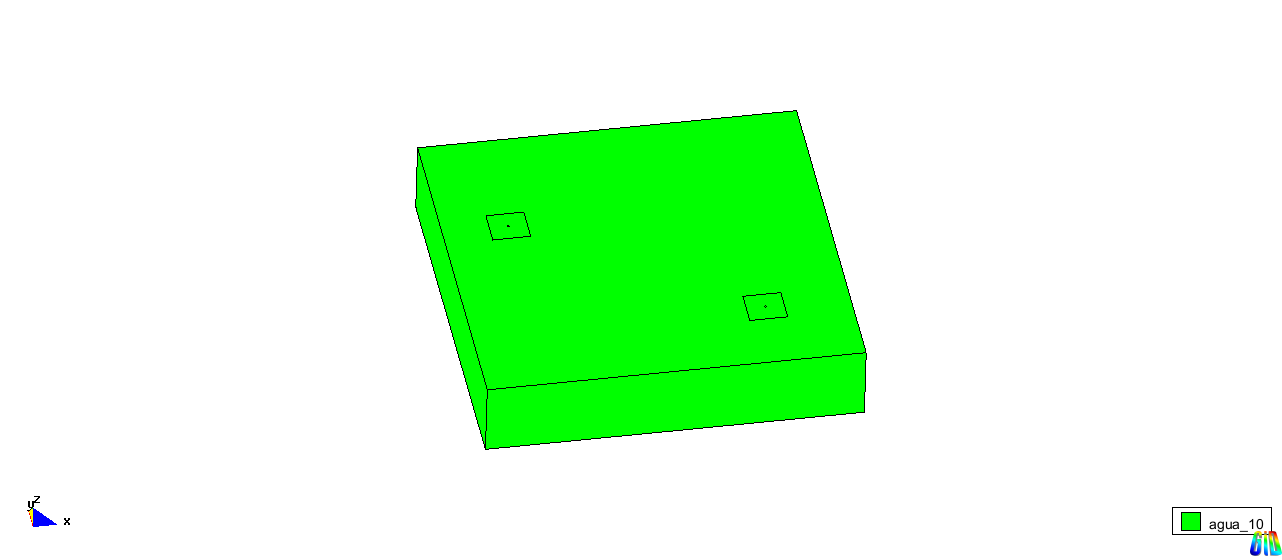
\includegraphics[scale=0.5]{img/100m/100_perspectiva_material_agua}}
\caption{Material Suelo asignado a la geometría}
\label{100_perspectiva_material_agua}
\end{figure}
%%%%%%%%%%%%%%%%%%%%%%%%%%%%%%%
\subsubsection{Material Wall o Pared}
En la ventana de contornos $\rightarrow$ fluidos, se asigno a las paredes de ambos pozos el contorno definido por defecto Wall. El tipo de contorno seleccionado fue el \emph{V fixWall} con el ángulo por defecto de $60°$. Este es el modelo elegido en Tdyn para simular el comportamiento del flujo en las paredes del dominio. Básicamente, impone que la velocidad en las superficies asignadas será nula, modelando así la pared del pozo por la que no existe penetración de agua hacia el interior del del mismo. En la figura \ref{100_condiciones_vfixwall_xz} se puede observar el material asignado a ambos pozos.
%
\begin{figure}[tbhp]
\centerline{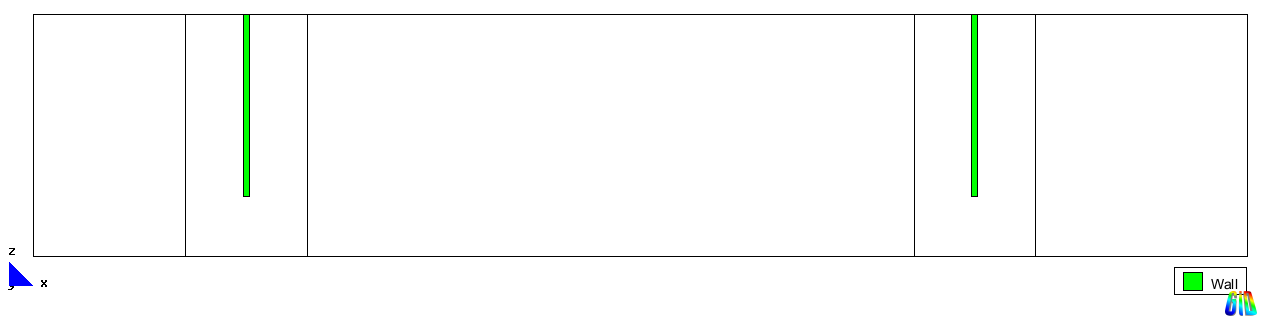
\includegraphics[scale=0.3]{img/100m/100_condiciones_vfixwall_xz}}
\caption{Material Wall o Pared asignado a la geometría}
\label{100_condiciones_vfixwall_xz}
\end{figure}
%
%%%%%%%%%%%%%%%%%%%%%%%%%%%%%%%%%%%%%%%%%%%%%%%%%%%%%%%%%%%%%%%%%%%%%%%%%%%%%%%%%%%%%%%%%%%%%%%%%%%
\subsection{Condiciones de borde}
Para fijar las condiciones de borde, se procedió mediante el menú datos $\Rightarrow$ condiciones $\Rightarrow$ ransol. Luego se selecciono la opción de asignación de propiedades a superficies y se procedió a fijar las diferentes condiciones:

\begin{figure}[tbhp]
\centerline{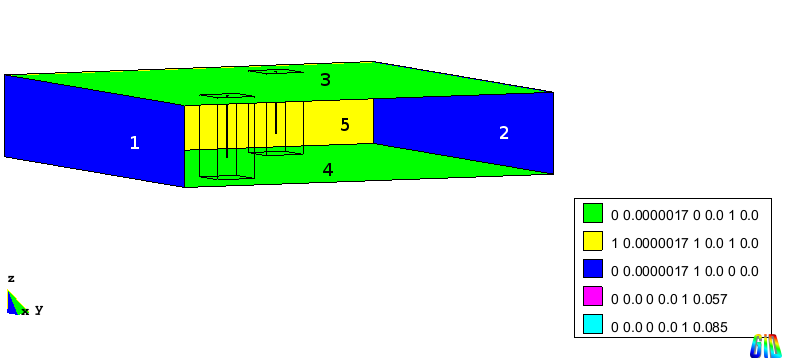
\includegraphics[scale=0.4]{img/100m/100_condiciones_fijar_velocidad_perspectiva_interior_leyendas}}
\caption{Velocidades Fijas}
\label{100_condiciones_fijar_velocidad_perspectiva_interior_leyendas}
\end{figure}
%%%%%%%%%%%%%%%%%%%%%%%%%%%%%%
\subsubsection{Fijar Velocidad}
Como se puede ver en la figura (\ref{100_condiciones_fijar_velocidad_perspectiva_interior_leyendas}) las condiciones asignadas a cada una de las superficies enumeradas son las siguientes:

\begin{enumerate}

\item Superficie 1 y 2:

\begin{eqnarray*}
Libre~V_x&=&0.0000017~[m/s]\\
Fija~V_y&=&0.0~[m/s]\\
Libre~V_z&=&0.0~[m/s]
\end{eqnarray*}
Observar, que en las superficies 1 y 2 marcadas en la figura (\ref{100_condiciones_fijar_velocidad_perspectiva_interior_leyendas}) se fija la velocidad $V_y$ a $0$, esto se hace con el objetivo de impedir que el fluido escape del dominio (impermeabilidad de las paredes laterales). En la dirección de $x$ y $y$ el movimiento es libre.

\item Superficie 3 y 4:

\begin{eqnarray*}
Libre~V_x&=&0.0000017~[m/s]\\
Libre~V_y&=&0.0~[m/s]\\
Fija~V_z&=&0.0~[m/s]
\end{eqnarray*}

En estas superficies se fija la velocidad $V_z$ a $0$. En la superficie marcada con el número 4 en la figura (\ref{100_condiciones_fijar_velocidad_perspectiva_interior_leyendas}), se lo hace para representar la impermeabilidad de la superficie inferior y superior del campo (acuífero confinado). En las direcciones de $x$ y $y$ el movimiento es libre.

\item Superficie 5:

\begin{eqnarray*}
Fija~V_x&=&0.0000017~[m/s]\\
Fija~V_y&=&0.0~[m/s]\\
Fija~V_z&=&0.0~[m/s]\\
\end{eqnarray*}

Se puede observar que en esta superficie, se fijan las velocidades en las 3 direcciones, $x$, $y$ y $z$. Esto, modela la entrada de agua que se desplaza en una sola dirección ($x$). Además ese desplazamiento es a la misma velocidad con el que se determino la constante de permeabilidad $k$ de la \emph{Ley de Darcy}.
\end{enumerate}
%%%%%%%%%%%%%%%%%%%%%%%%%%%%%%
Para modelar la extracción de agua de los pozos, se fijo la velocidad en el eje de las $Z$ con el valor calculado en la sección \ref{subseccion_transformacion_caudal} para cada uno de los pozos:
%
\begin{enumerate}
\item Pozo 1:
\begin{eqnarray*}
Libre~V_x&=&0.0~[m/s]\\
Libre~V_y&=&0.0~[m/s]\\
Fija~V_z&=&0.085~[m/s]\\
\end{eqnarray*}
%
\item Pozo 2:
\begin{eqnarray*}
Libre~V_x&=&0.0~[m/s]\\
Libre~V_y&=&0.0~[m/s]\\
Fija~V_z&=&0.057~[m/s]\\
\end{eqnarray*}
\end{enumerate}
%
En la figura (\ref{100_condiciones_fijar_velocidad_fondo_pozos}) y (\ref{fondo_pozos_detalles}) se puede ver la condición asignada en color cian y magenta, para el pozo 1 y 2 respectivamente.

\begin{figure}[tbhp]
\centerline{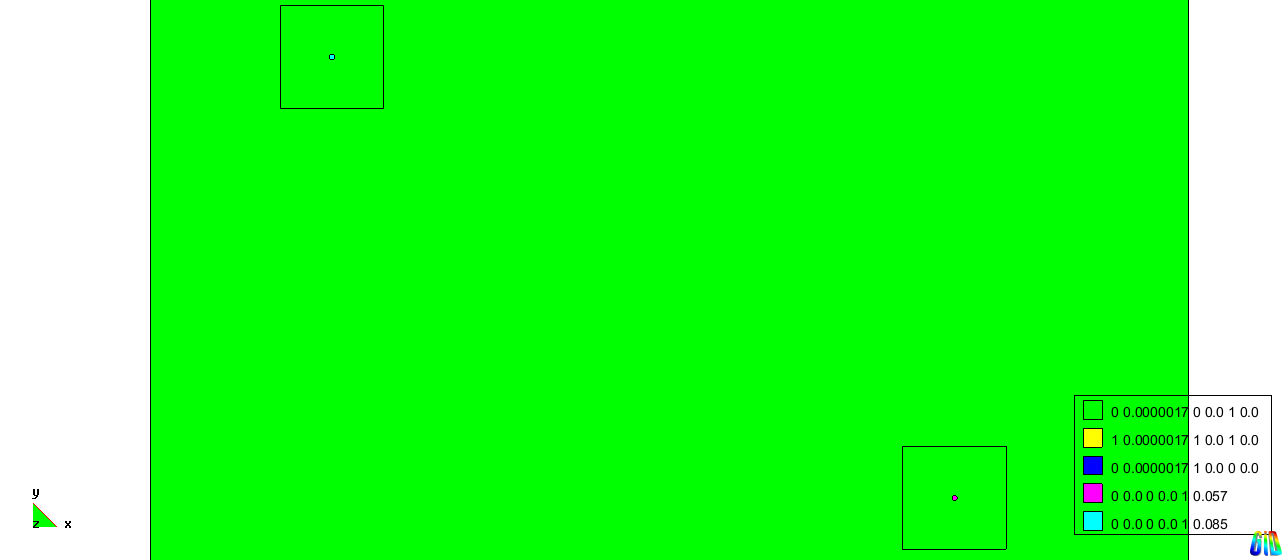
\includegraphics[scale=0.4]{img/100m/100_condiciones_fijar_velocidad_fondo_pozos}}
\caption{Condición Fijar Velocidad para los pozos de bombeo}
\label{100_condiciones_fijar_velocidad_fondo_pozos}
\end{figure}
%%%%%%%%%%%%%%%%%%%%%%%%%%%%%%%%%%%%%%%%%%%%%%%%%%%%%%%%%%%%%%%%%%%%%%%%%%%%%%%%%%%%%%%%%%%%%%%%%%%
\begin{figure}[htbp] 
\centering 
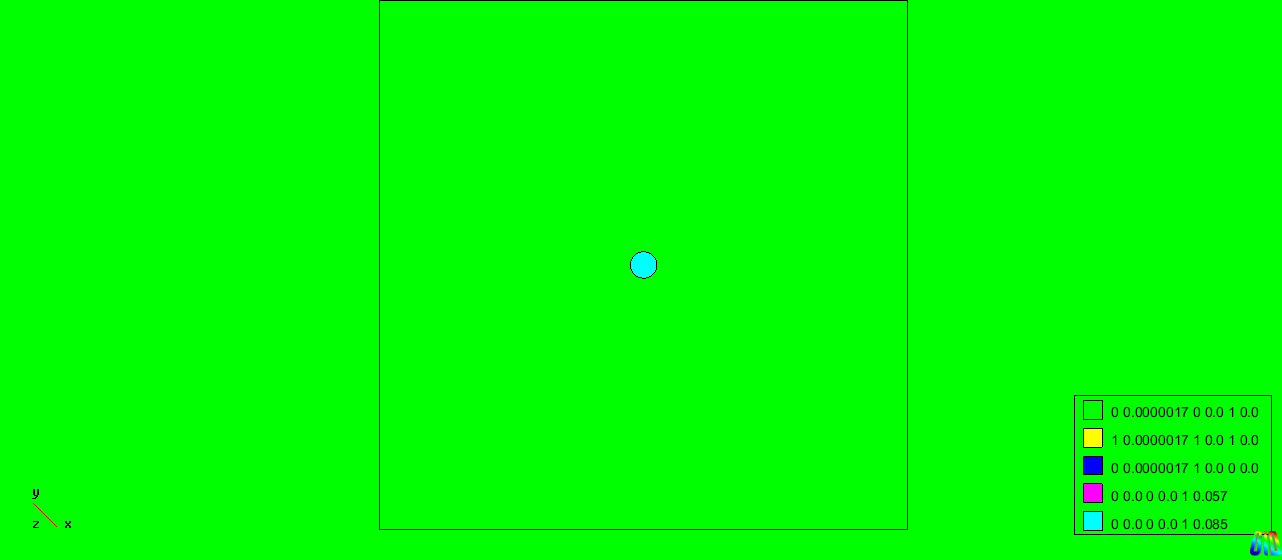
\includegraphics[scale=0.25]{img/100m/100_condiciones_fijar_velocidad_fondo_pozos_arriba_izquierda} 
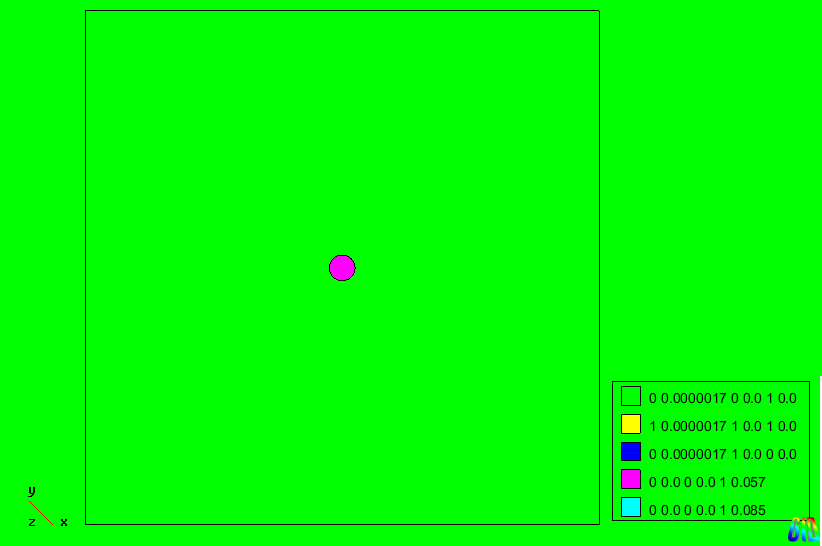
\includegraphics[scale=0.25]{img/100m/100_condiciones_fijar_velocidad_fondo_pozos_abajo_derecha}
\caption{Vista en detalle de la Figura (\ref{100_condiciones_fijar_velocidad_fondo_pozos})} 
\label{fondo_pozos_detalles} 
\end{figure} 
%%%%%%%%%%%%%%%%%%%%%%%%%%%%%%
\subsubsection{Fijar Presión}
En la figura \ref{100_condiciones_presion0} se puede observar que se fijó un valor de referencia para la presión en la superficie del extremo final de salida del campo con valor igual a $0.0~\left[Pa\right]$. Esto significa que los resultados que obtendremos para la presión serán relativos a esta condición.

\begin{figure}[tbhp]
\centerline{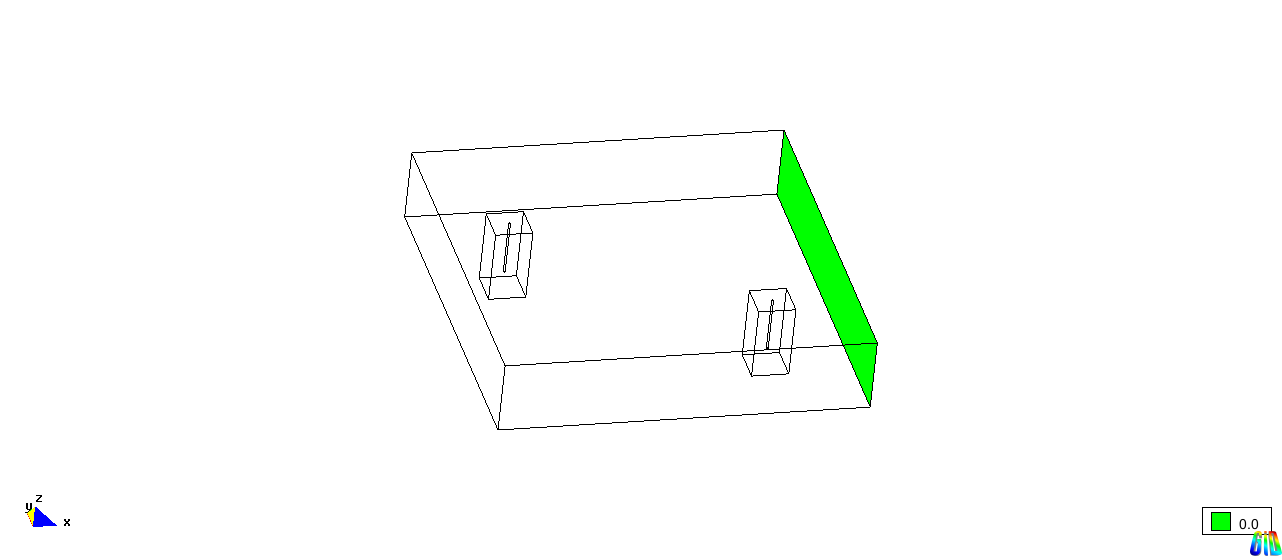
\includegraphics[scale=0.5]{img/100m/100_condiciones_presion0}}
\caption{Condición fija de presión}
\label{100_condiciones_presion0}
\end{figure}
%%%%%%%%%%%%%%%%%%%%%%%%%%%%%%
\subsection{Mallado}
Para el mallado, se asignaron diferentes tamaños a las superficies debido a que se deseó obtener un mayor detalle en las cercanías de ambos pozos. Para ello se subdividió el dominio como se muestra en las figuras (\ref{100_xy_cotas}) y (\ref{100_xz_cotas}) para \emph{G1} y en las figuras (\ref{200_xy_cotas}) y (\ref{200_xz_cotas}) para \emph{G2}. Luego, se aplicó una malla no estructurada de diferentes tamaños para las diferentes entidades, como se puede ver en las figuras (\ref{100_perspec_tam_malla}) y (\ref{100_xz_tam_malla}) en el caso de \emph{G1} y en las figuras (\ref{200_xy_tam_malla}) y (\ref{200_xz_tam_malla}) en el caso de \emph{G2}.

Además, en las preferencias de mallado de Gid (Utilidades $\rightarrow$ preferencias $\rightarrow$ pestaña malla), se fijó la transición de tamaños no estructurados a $0.3$.
%
\begin{figure}[tbhp]
\centerline{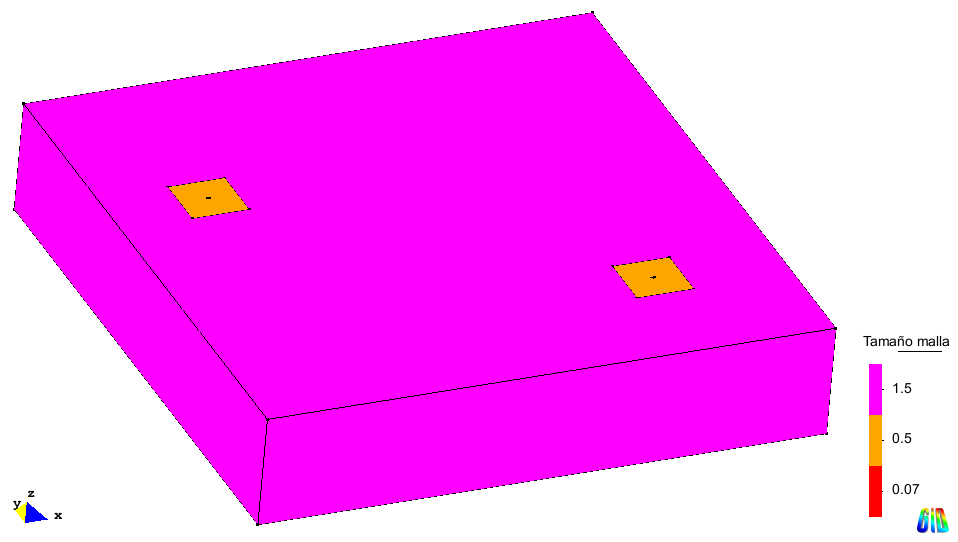
\includegraphics[scale=0.35]{img/100m/100_perspec_tam_malla}}
\caption{Tamaños de los elementos de la malla \emph{G1}- Vista en perspectiva}
\label{100_perspec_tam_malla}
\end{figure}
%
\begin{figure}[tbhp]
\centerline{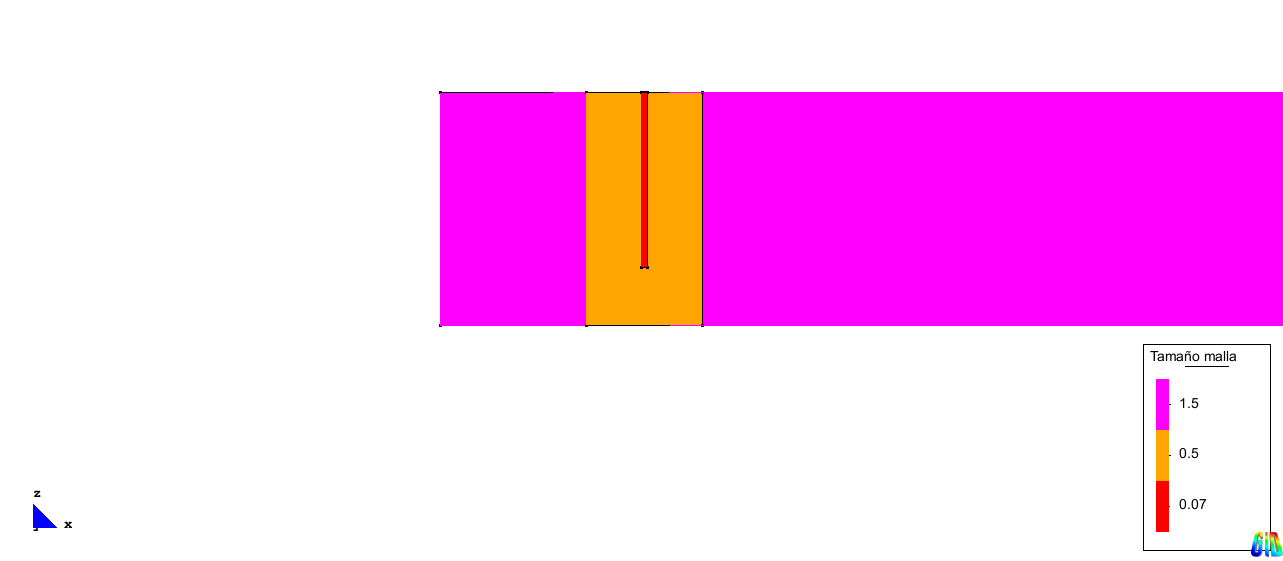
\includegraphics[scale=0.4]{img/100m/100_xz_tam_malla}}
\caption{Tamaños de los elementos de la malla \emph{G1}- Vista plano XZ}
\label{100_xz_tam_malla}
\end{figure}
%%
\begin{figure}[tbhp]
\centerline{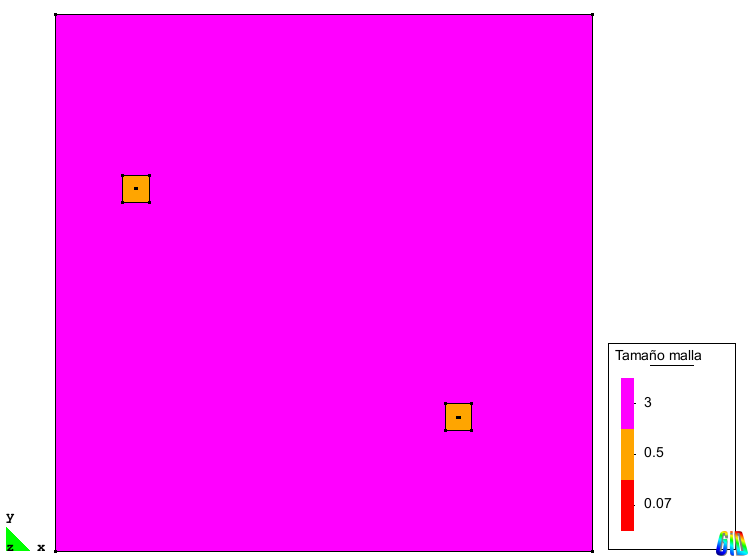
\includegraphics[scale=0.4]{img/200m/200_xy_tam_malla}}
\caption{Tamaños de los elementos de la malla para \emph{G2}- Vista plano XY}
\label{200_xy_tam_malla}
\end{figure}
%
\begin{figure}[tbhp]
\centerline{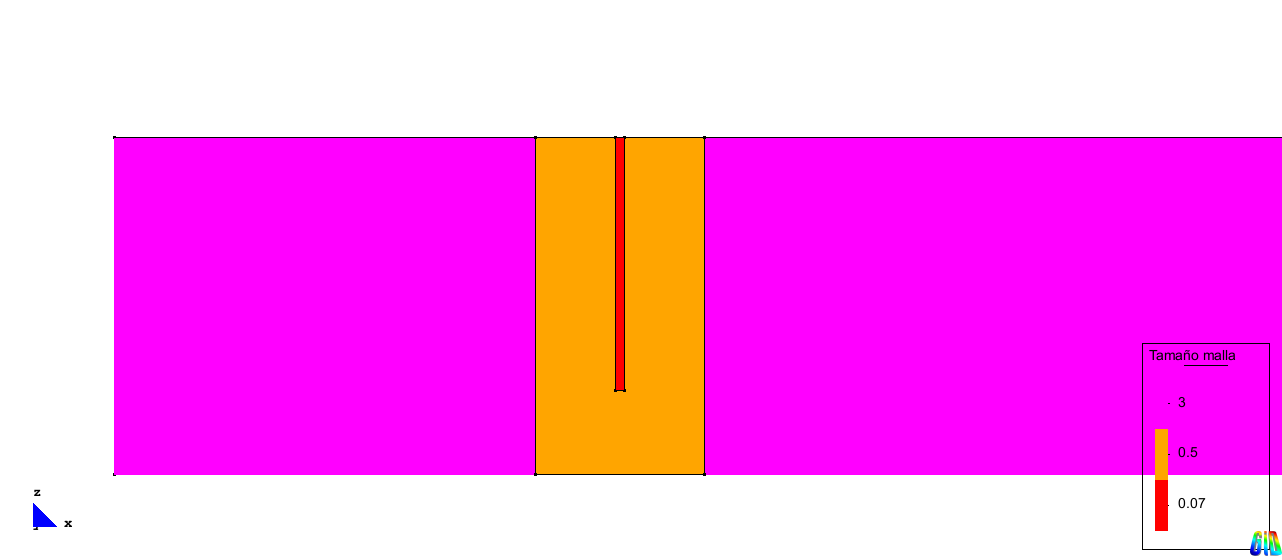
\includegraphics[scale=0.4]{img/200m/200_xz_tam_malla}}
\caption{Tamaños de los elementos de la malla \emph{G2}- Vista plano XZ}
\label{200_xz_tam_malla}
\end{figure}
%
%
\begin{table}[tbhp]
\begin{center}\begin{tabular}{ccc}
\hline \textbf{Tipo/Geometría} & \textbf{G1} & \textbf{G2} \\ 
\hline Número de nodos: & 122586 & 157619 \\ 
\hline Número de tetraedros: & 659027 & 851671\\ 
\hline Número de triángulos: & 60952  & 70582 \\ 
\hline Número de elementos totales: & 719979 & 922253 \\ 
\hline 
\label{tabla_lista_elementos}
\end{tabular}\end{center}
\caption{Cantidad de nodos, tetraedros, triángulos y elementos totales para \emph{G1} y \emph{G2}}
\end{table}
%
En la tabla (\ref{tabla_lista_elementos}), se presentan los tipos y cantidades de elementos con los que esta conformado cada una de las geometrías:
%
La calidad de la malla para \emph{G1} y \emph{G2} se muestra en la Fig. (\ref{calidad_malla_g1}) y (\ref{calidad_malla_g2}) respectivamente.
%
\begin{figure}[htbp] 
\centering 
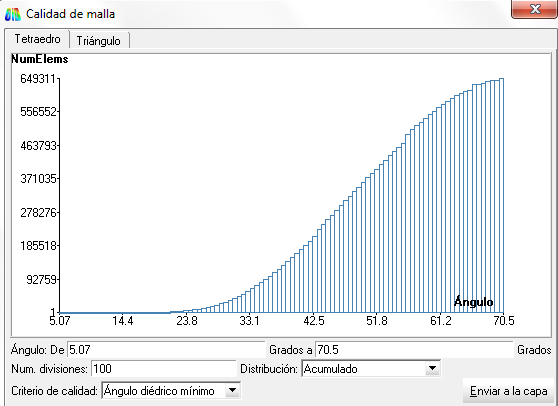
\includegraphics[width=0.45\textwidth]{img/100m/100_calidad_malla_tetraedros} 
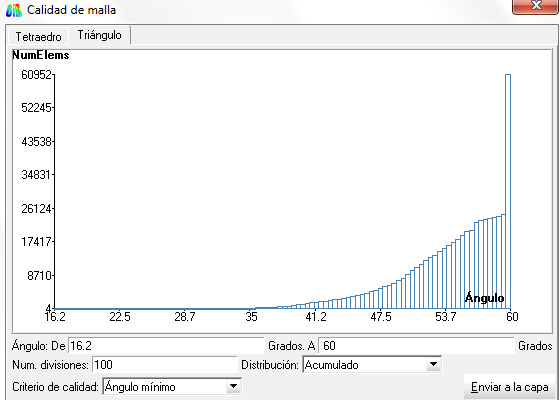
\includegraphics[width=0.45\textwidth]{img/100m/100_calidad_malla_triangulos}
\caption{Calidad de la Malla para \emph{G1}} 
\label{calidad_malla_g1} 
\end{figure} 
%
%
\begin{figure}[htbp] 
\centering 
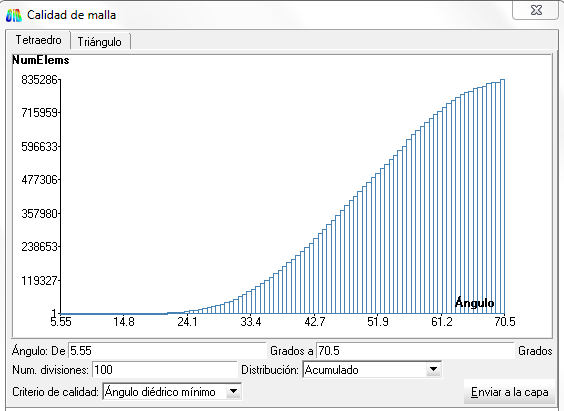
\includegraphics[width=0.45\textwidth]{img/200m/200_calidad_malla_tetraedros} 
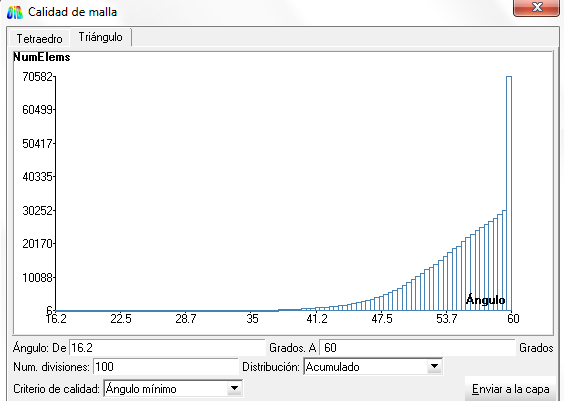
\includegraphics[width=0.45\textwidth]{img/200m/200_calidad_malla_triangulos}
\caption{Calidad de la Malla para \emph{G2}} 
\label{calidad_malla_g2} 
\end{figure} 
%
Finalmente, en las figuras (\ref{100_xy_contorno_malla}) y (\ref{200_xy_contorno_malla}) se puede observar la malla generada.
\begin{figure}[tbhp]
\centerline{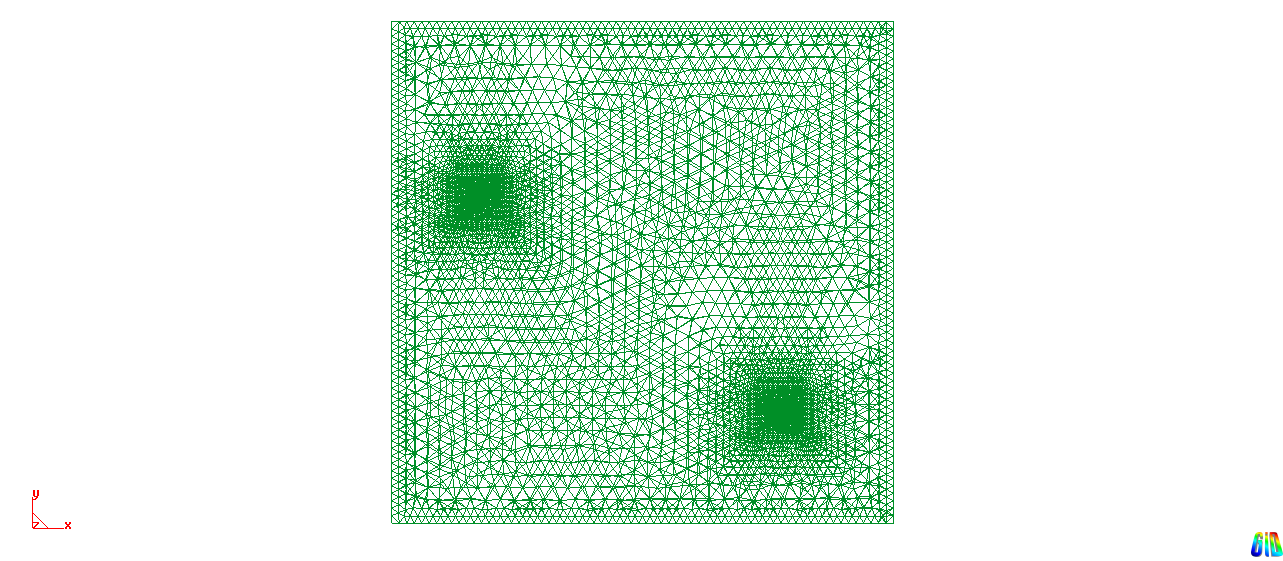
\includegraphics[scale=0.4]{img/100m/100_xy_contorno_malla}}
\caption{Mallado generada para \emph{G1}- Vista plano XY}
\label{100_xy_contorno_malla}
\end{figure}
%
\begin{figure}[tbhp]
\centerline{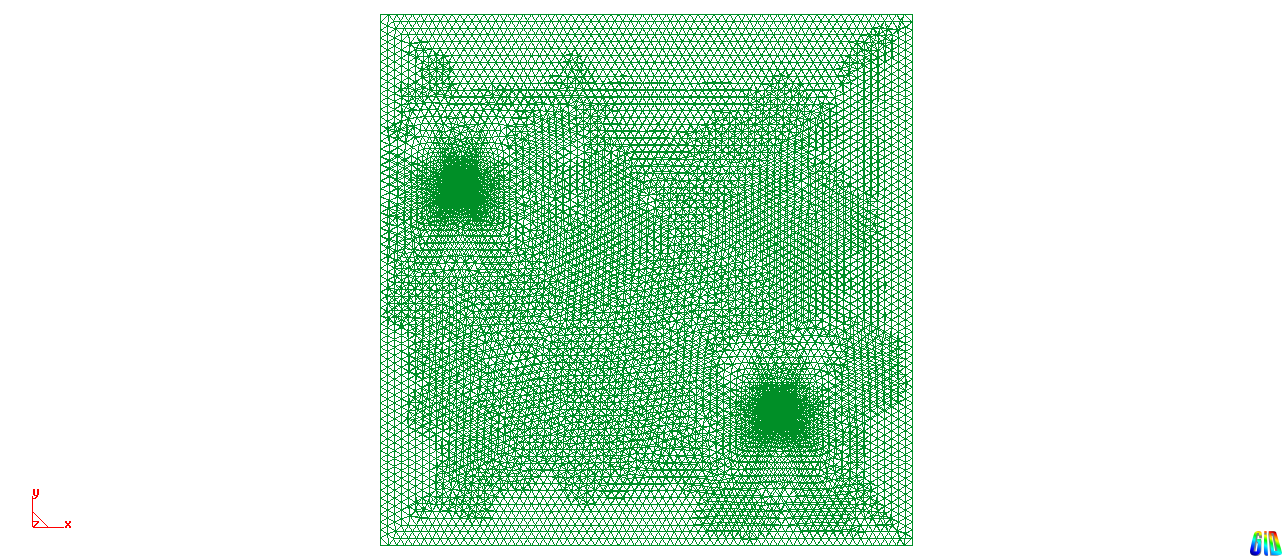
\includegraphics[scale=0.4]{img/200m/200_xy_contorno_malla}}
\caption{Mallado generada para \emph{G2}- Vista plano XY}
\label{200_xy_contorno_malla}
\end{figure}
%
%%%%%%%%%%%%%%%%%%%%%%%%%%%%%%%%%%%%%%%%%%%%%%%%%%%%%%%%%%%%%%%%%%%%%%%%%%%%%%%%%%%%%%%%%%%%%%%%%%%
%%%%%%%%%%%%%%%%%%%%%%%%%%%%%%%%%%%%%%%%%%%%%%%%%%%%%%%%%%%%%%%%%%%%%%%%%%%%%%%%%%%%%%%%%%%%%%%%%%%
\subsection{Ejecución}
Para la simulación, se hicieron 1000 pasos con un paso de tiempo $\Delta t=10~[s]$ lo que equivale 2 horas, 46 minutos y 40 segundos de extracción de agua por parte de las bombas.
%%%%%%%%%%%%%%%%%%%%%%%%%%%%%%%%%%%%%%%%%%%%%%%%%%%%%%%%%%%%%%%%%%%%%%%%%%%%%%%%%%%%%%%%%%%%%%%%%%
%%%%%%%%%%%%%%%%%%%%%%%%%%%%%%%%%%%%%%%%%%%%%%%%%%%%%%%%%%%%%%%%%%%%%%%%%%%%%%%%%%%%%%%%%%%%%%%%%%
%%%%%%%%%%%%%%%%%%%%%%%%%%%%%%%%%%%%%%%%%%%%%%%%%%%%%%%%%%%%%%%%%%%%%%%%%%%%%%%%%%%%%%%%%%%%%%%%%%
\section{Resultados}
A continuación se presentan los resultados de la simulación para el problema
%100_grafico_presion_velocidad_x_centro_pozos_distancia05.png
%100_grafico_presion_velocidad_x_centro_pozos_distancia0.png
%100_grafico_presion_velocidad_x_centro_pozos_distancia1.png
\subsection{Resultados para \emph{G1}}
En la figura (\ref{100_xy_vectores}) se pueden observar los vectores de velocidad en el plano $XY$, que se desplazan de derecha a izquierda, esto es debido a la condición de borde impuesta en la pared 5 de la figura (\ref{100_condiciones_fijar_velocidad_perspectiva_interior_leyendas}). También se puede ver que los vectores tienden hacia la posición de las bombas de succión de agua, lo cual referencia a las condiciones impuestas que se pueden ver en al figura (\ref{100_condiciones_fijar_velocidad_fondo_pozos}).
%
\begin{figure}[tbhp]
\centerline{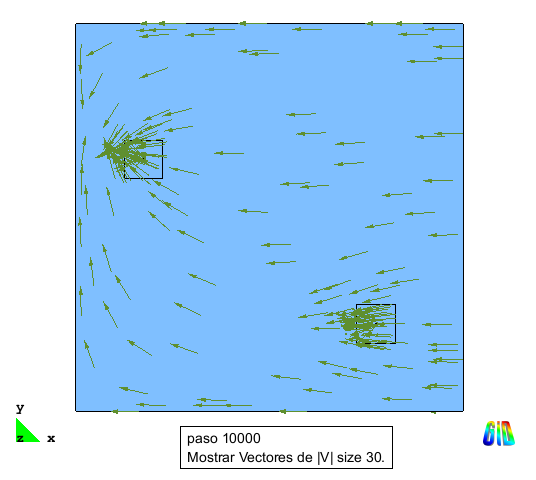
\includegraphics[scale=0.5]{img/100m/resul/100_xy_vectores}}
\caption{Vectores para \emph{G1}- Vista plano XY}
\label{100_xy_vectores}
\end{figure}
%
\\
En la figura (\ref{100_XZ_presion_corte_centro}), se puede observar la presión que existe en ambas bocas de succión de ambos pozos, lo cual se obtuvo mediante la realización de un corte que pase por el centro de cada uno de los mismos. En la figura (\ref{100_XZ_presion_corte_centro_pozo1}), se observa una depresión mayor que en (\ref{100_XZ_presion_corte_centro_pozo2}). Esto se debe, a que el pozo 1, posee una velocidad de extracción de agua mayor, que la del pozo 2.
%
\begin{figure}[tbhp]
   \centering
   %%----primera subfigura----
   \subfloat[]{
        \label{100_XZ_presion_corte_centro_pozo1}         %% Etiqueta para la primera subfigura
        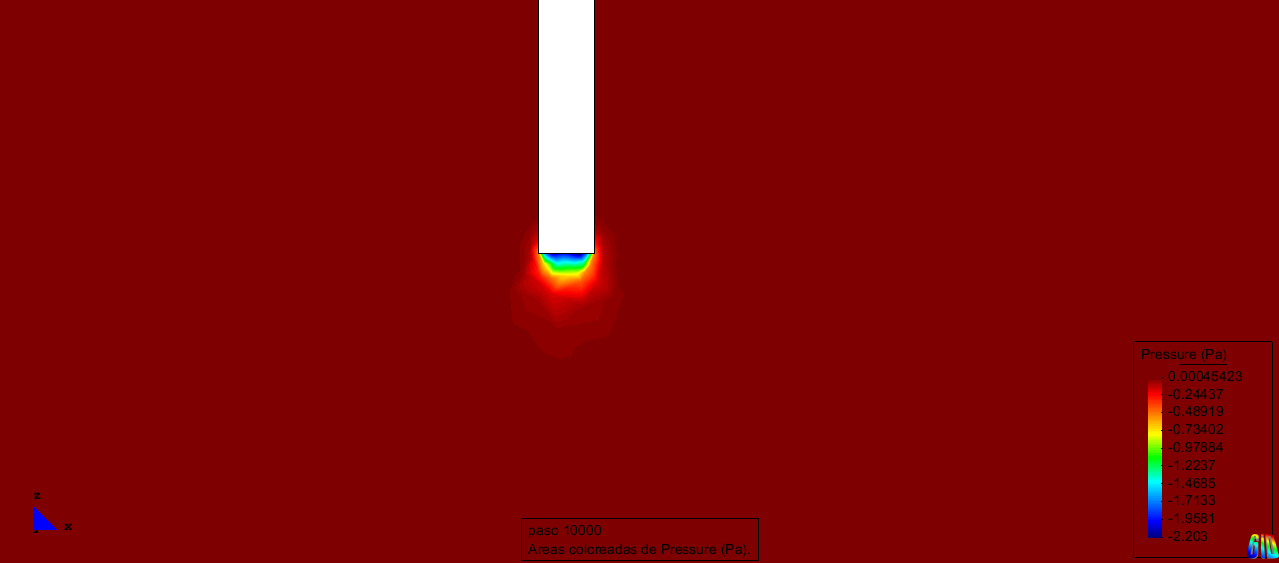
\includegraphics[scale=0.4]{img/100m/resul/100_XZ_presion_corte_centro_pozo1}}
   \hspace{0.1\linewidth}
   %%----segunda subfigura----
   \subfloat[]{
        \label{100_XZ_presion_corte_centro_pozo2}         %% Etiqueta para la segunda subfigura
        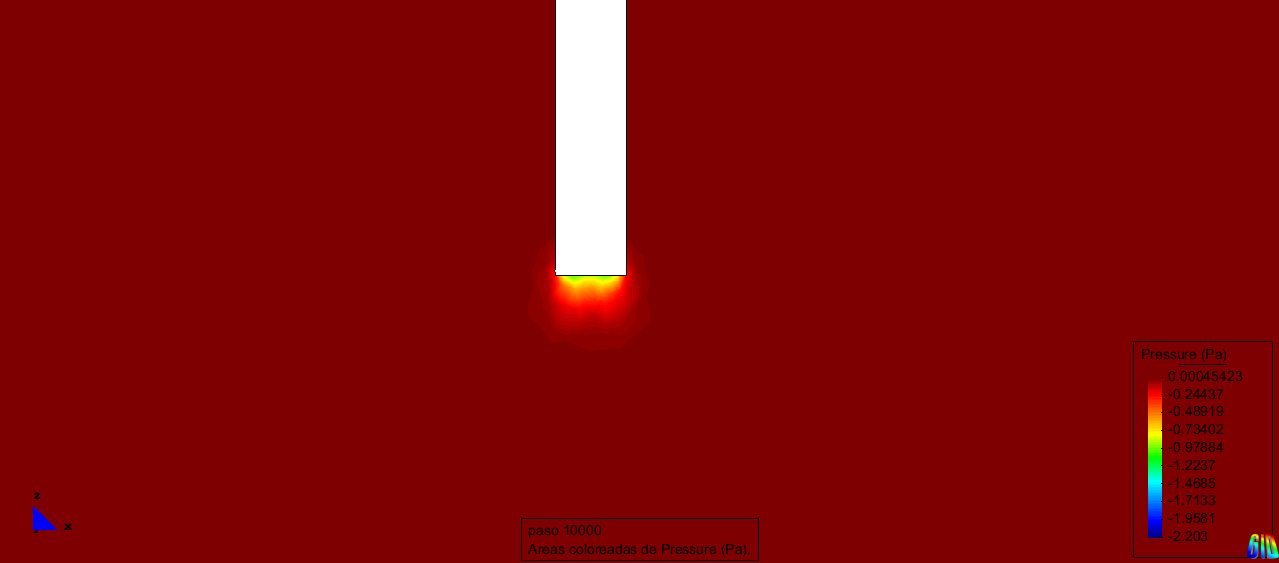
\includegraphics[scale=0.4]{img/100m/resul/100_XZ_presion_corte_centro_pozo2}}
    \caption{Corte a través del centro de ambos pozos para \emph{G1} - Vista en el plano XZ - (\ref{100_XZ_presion_corte_centro_pozo1}) Presión pozo 1. - (\ref{100_XZ_presion_corte_centro_pozo2})  Presión pozo 2.}
   \label{100_XZ_presion_corte_centro}                %% Etiqueta para la figura entera
\end{figure}
%
\\
En la figura (\ref{100_XZ_velocidad_corte_centro_pozos}), se observa la velocidad en las bases de los pozos, notándose un mayor valor del módulo en la fig. (\ref{100_XZ_velocidad_corte_centro_pozo1}) que en (\ref{100_XZ_velocidad_corte_centro_pozo2}), ya que como se describió antes, la velocidad de pozo 1 es de $0.085~[m/s]$, en tanto que la del pozo 2 (es levemente menor) es igual a $0.057~[m/s]$.
%
%corte centro pozos:
\begin{figure}[tbhp]
   \centering
   %%----primera subfigura----
   \subfloat[]{
        \label{100_XZ_velocidad_corte_centro_pozo1}         %% Etiqueta para la primera subfigura
        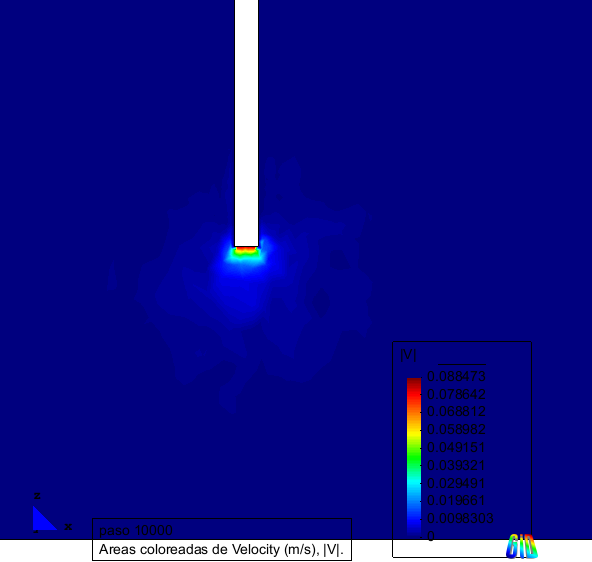
\includegraphics[scale=0.4]{img/100m/resul/100_XZ_velocidad_corte_centro_pozo1}}
   \hspace{0.1\linewidth}
   %%----segunda subfigura----
   \subfloat[]{
        \label{100_XZ_velocidad_corte_centro_pozo2}         %% Etiqueta para la segunda subfigura
        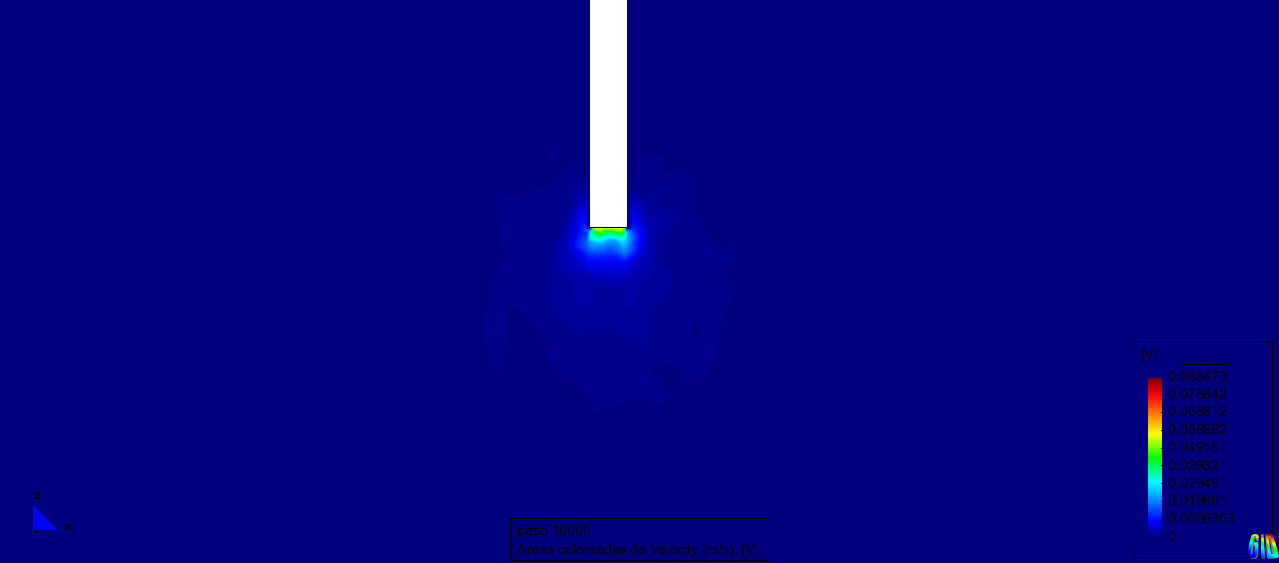
\includegraphics[scale=0.4]{img/100m/resul/100_XZ_velocidad_corte_centro_pozo2}}
    \caption{Corte a través del centro de ambos pozos para \emph{G1} - Vista en el plano XZ - (\ref{100_XZ_velocidad_corte_centro_pozo1}) Módulo de velocidad pozo 1. - (\ref{100_XZ_velocidad_corte_centro_pozo2}) Módulo de velocidad pozo 2.}
   \label{100_XZ_velocidad_corte_centro_pozos}                %% Etiqueta para la figura entera
\end{figure}
%
\\
En las figuras (\ref{100_presion_horizontal}) y (\ref{100_velocidad_horizontal}), se observa la presión y velocidad respectivamente, en un corte transversal del dominio unido por la linea de coordenadas $(x_1,y_1,z_1)=(0,50,0)$ y $(x_2,y_2,z_2)=(100,50,0)$; de forma similar, en las figuras (\ref{100_velocidad_presion_vertical}) y (\ref{100_velocidad_vertical}) se puede observar presión y velocidad respectivamente, en un corte transversal del dominio unido por la linea de coordenadas $(x_1,y_1,z_1)=(50,0,0)$ y $(x_2,y_2,z_2)=(50,100,0)$;
%corte horizontal:
\begin{figure}[tbhp]
   \centering
   %%----primera subfigura----
   \subfloat[]{
        \label{100_presion_horizontal}         %% Etiqueta para la primera subfigura
        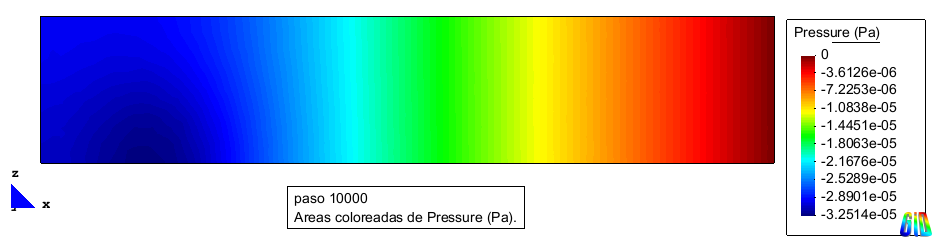
\includegraphics[scale=0.4]{img/100m/resul/100_XZ_presion_corte_horizontal}}
   \hspace{0.1\linewidth}
   %%----segunda subfigura----
   \subfloat[]{
        \label{100_velocidad_horizontal}         %% Etiqueta para la segunda subfigura
        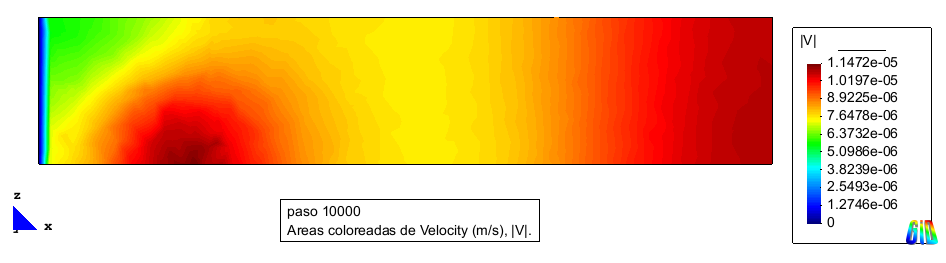
\includegraphics[scale=0.4]{img/100m/resul/100_XZ_velocidad_corte_horizontal}}
    \caption{Corte en $(x_1,y_1,z_1)=(0,50,0)$ hasta $(x_2,y_2,z_2)=(100,50,0)$ para \emph{G1} - Vista en el plano XZ - (\ref{100_presion_horizontal}) Presión. - (\ref{100_velocidad_horizontal}) Módulo de Velocidad.}
   \label{100_velocidad_presion_horizontal}                %% Etiqueta para la figura entera
\end{figure}
%
%
\begin{figure}[tbhp]
   \centering
   %%----primera subfigura----
   \subfloat[]{
        \label{100_presion_vertical}         %% Etiqueta para la primera subfigura
        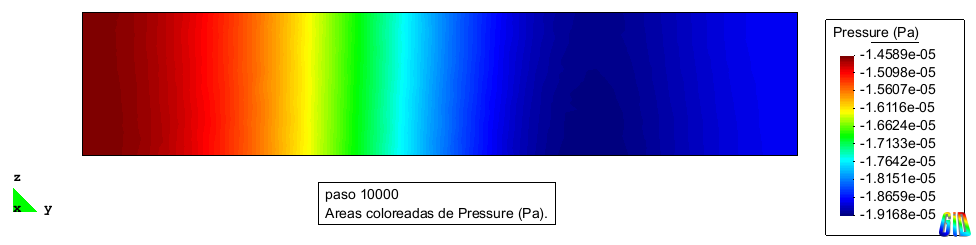
\includegraphics[scale=0.4]{img/100m/resul/100_ZY_presion_corte_vertical}}
   \hspace{0.1\linewidth}
   %%----segunda subfigura----
   \subfloat[]{
        \label{100_velocidad_vertical}         %% Etiqueta para la segunda subfigura
        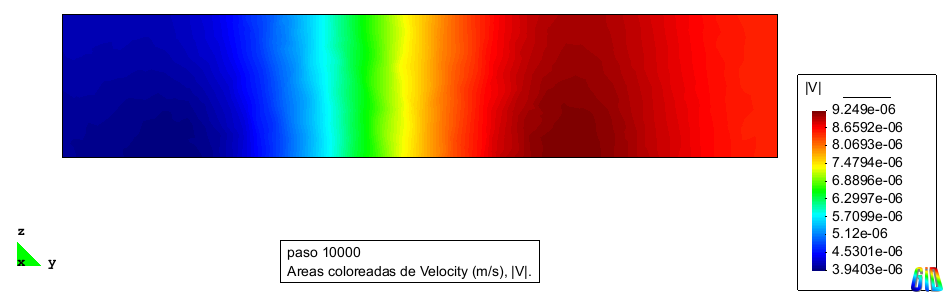
\includegraphics[scale=0.4]{img/100m/resul/100_ZY_velocidad_corte_vertical}}
    \caption{Corte en $(x_1,y_1,z_1)=(50,0,0)$ hasta $(x_2,y_2,z_2)=(50,100,0)$ para \emph{G1} - Vista en el plano YZ - (\ref{100_presion_vertical}) Presión. - (\ref{100_velocidad_vertical}) Módulo de Velocidad.}
   \label{100_velocidad_presion_vertical}                %% Etiqueta para la figura entera
\end{figure}
%%%%%%%%%%%%%%%%%%%%%%%%%%%%%%%%%%%%%%%%%%%%%%%%%%%%%%%%%%
\\
También se realizaron cortes como se puede observar en la figura (\ref{perfiles}), sobre los cuales se obtuvieron las gráficas de borde (Eje X: Variación en X, Eje Y: Presión/Velocidad) que se representan en las figuras (\ref{100_grafico_velocidad_presion_centro_pozos_distancia0}), (\ref{100_grafico_velocidad_presion_centro_pozos_distancia05}) y (\ref{100_grafico_velocidad_presion_centro_pozos_distancia1}) para \emph{G1}; y (\ref{200_grafico_velocidad_presion_centro_pozos_distancia0}),(\ref{200_grafico_velocidad_presion_centro_pozos_distancia05}) y (\ref{200_grafico_velocidad_presion_centro_pozos_distancia1}) para \emph{G2}.

\begin{figure}[tbhp]
\centerline{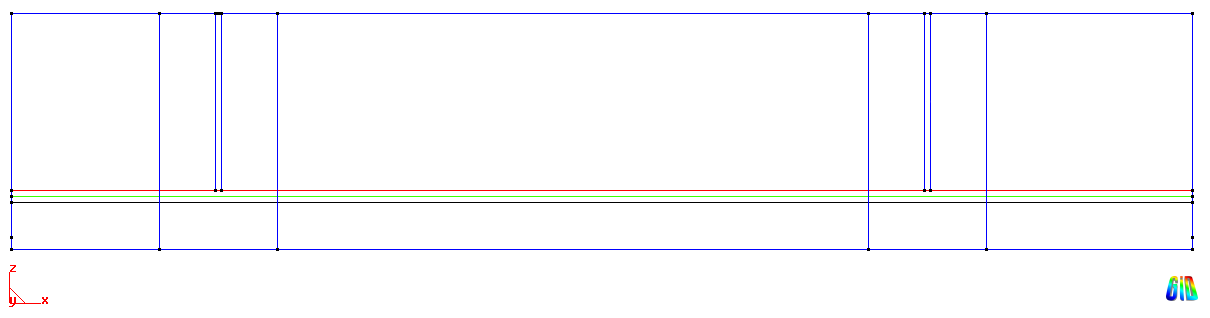
\includegraphics[scale=0.4]{img/200m/perfiles}}
\caption{\\\textbf{Linea roja:} (situada sobre la base de los pozos) a partir de la cuál se obtuvieron las Gráficas de borde de la Figura (\ref{100_grafico_velocidad_presion_centro_pozos_distancia0}) y (\ref{200_grafico_velocidad_presion_centro_pozos_distancia0}).\\
\textbf{Linea verde:} (situada a $0.5~[m]$ de la base de los pozos) a partir de la cuál se obtuvieron las Gráficas de borde de la Figura (\ref{100_grafico_velocidad_presion_centro_pozos_distancia05}) y (\ref{200_grafico_velocidad_presion_centro_pozos_distancia05}).
\\\textbf{Linea negra:} (situada a $1.0~[m]$ de la base de los pozos) a partir de la cuál se obtuvieron las Gráficas de borde de la Figura (\ref{100_grafico_velocidad_presion_centro_pozos_distancia1}) y (\ref{200_grafico_velocidad_presion_centro_pozos_distancia1}).}
\label{perfiles}
\end{figure}

%graficos00:
\begin{figure}[tbhp]
   \centering
   %%----primera subfigura----
   \subfloat[]{
        \label{100_grafico_presion_x_centro_pozos_distancia0}         %% Etiqueta para la primera subfigura
        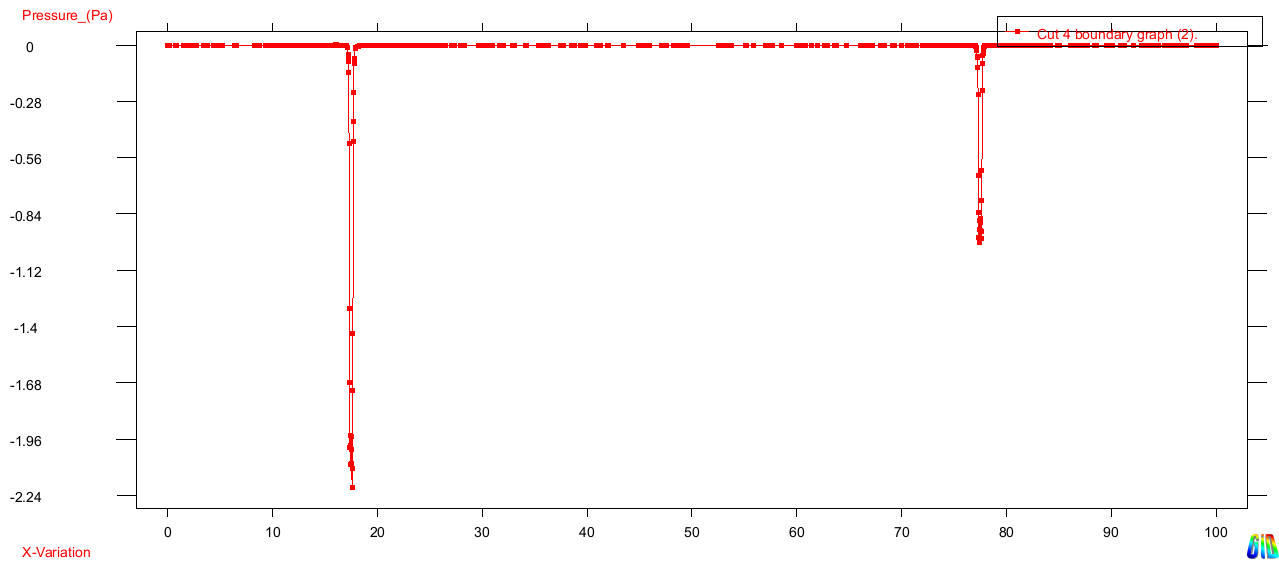
\includegraphics[scale=0.3]{img/100m/grf/100_grafico_presion_x_centro_pozos_distancia0}}
   \hspace{0.1\linewidth}
   %%----segunda subfigura----
   \subfloat[]{
        \label{100_grafico_velocidad_x_centro_pozos_distancia0}         %% Etiqueta para la segunda subfigura
        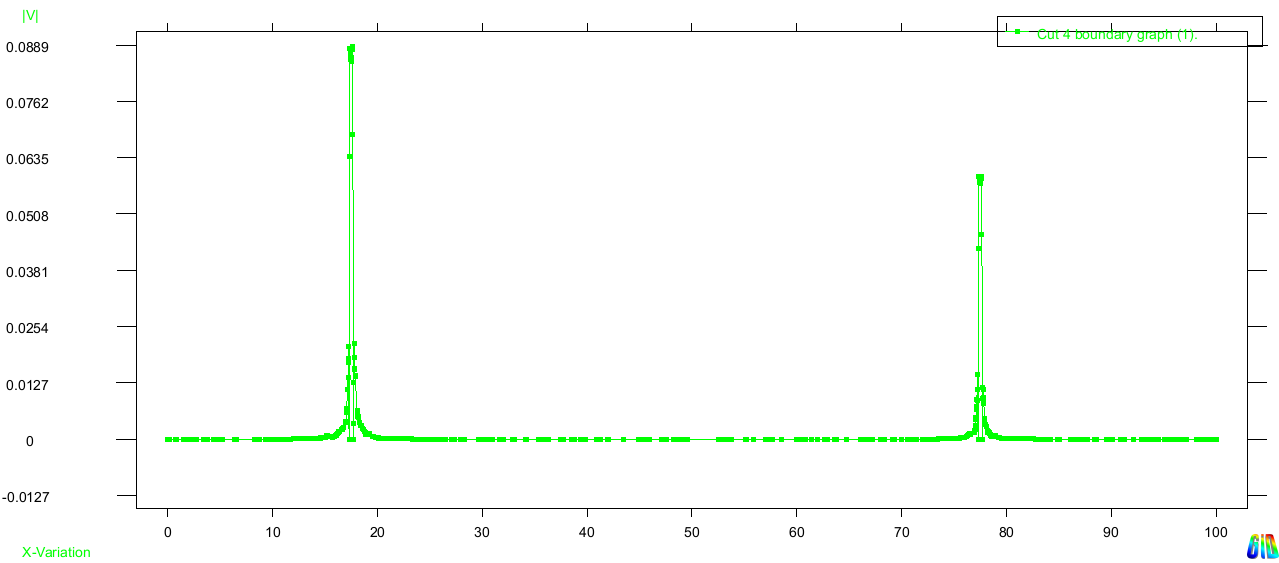
\includegraphics[scale=0.3]{img/100m/grf/100_grafico_velocidad_x_centro_pozos_distancia0}}
    \caption{Perfil de presión y velocidad para los pozos 1 y 2 de \emph{G1} situados sobre la base de los pozos. (\ref{100_grafico_presion_x_centro_pozos_distancia0}) Posición en $x$ vs. presión. - (\ref{100_grafico_velocidad_x_centro_pozos_distancia0}) Posición en $x$ vs. Módulo de Velocidad.}
   \label{100_grafico_velocidad_presion_centro_pozos_distancia0}                %% Etiqueta para la figura entera
\end{figure}
%
%graficos05:
\begin{figure}[tbhp]
   \centering
   %%----primera subfigura----
   \subfloat[]{
        \label{100_grafico_presion_x_centro_pozos_distancia05}         %% Etiqueta para la primera subfigura
        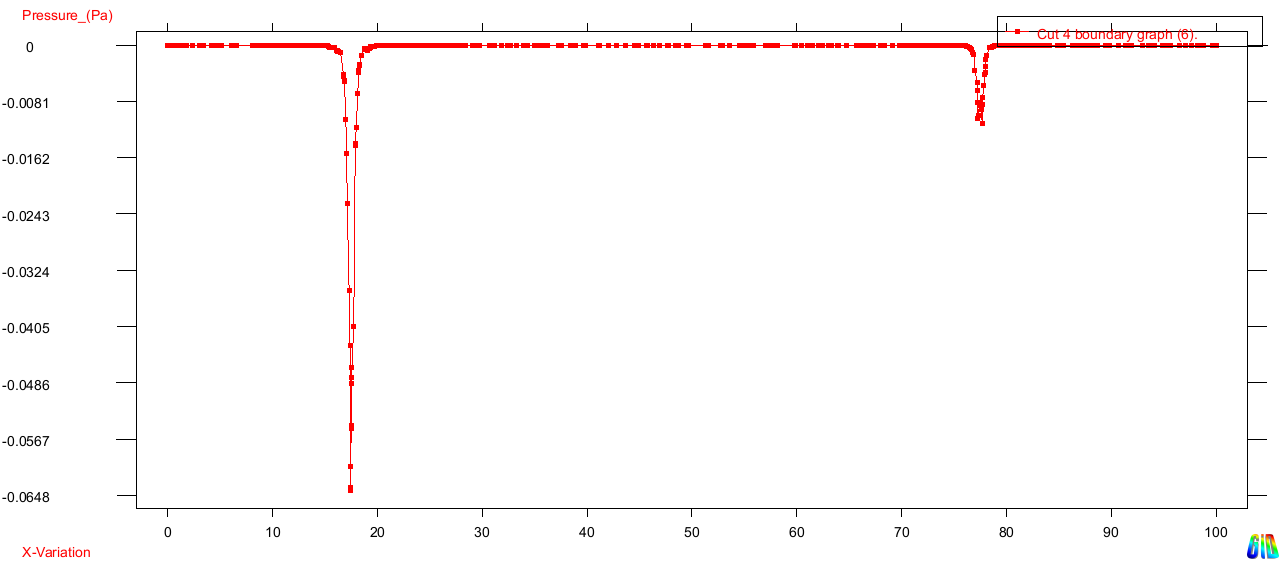
\includegraphics[scale=0.3]{img/100m/grf/100_grafico_presion_x_centro_pozos_distancia05}}
   \hspace{0.1\linewidth}
   %%----segunda subfigura----
   \subfloat[]{
        \label{100_grafico_velocidad_x_centro_pozos_distancia05}         %% Etiqueta para la segunda subfigura
        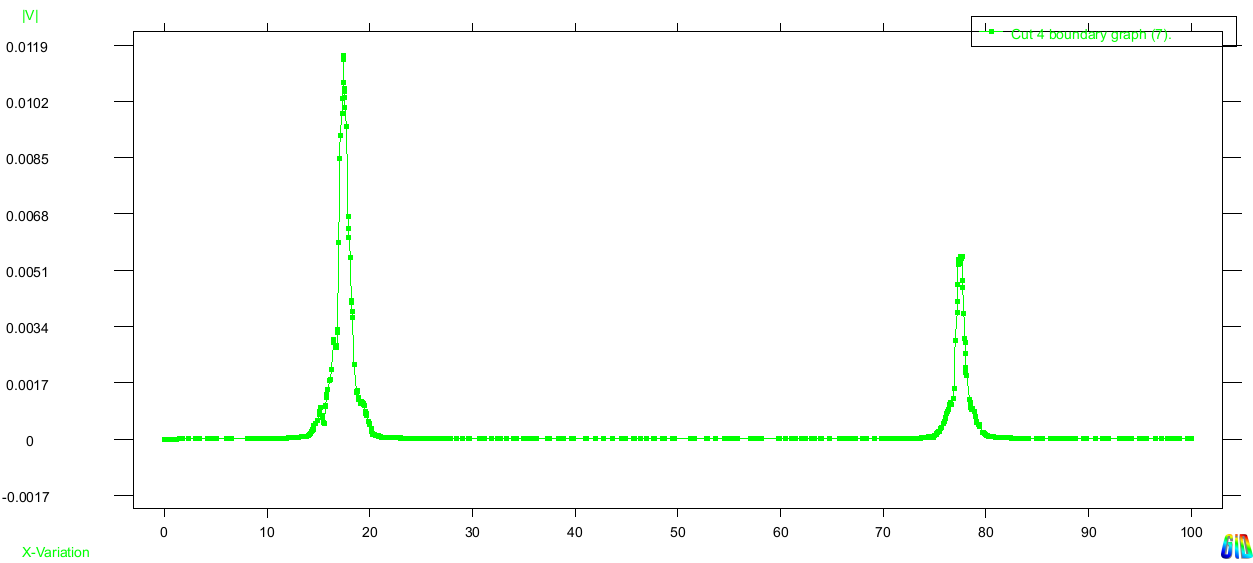
\includegraphics[scale=0.3]{img/100m/grf/100_grafico_velocidad_x_centro_pozos_distancia05}}
    \caption{Perfil de presión y velocidad para los pozos 1 y 2 de \emph{G1} situados a $0.5~[m]$ en dirección $-z$ de la base de los pozos. (\ref{100_grafico_presion_x_centro_pozos_distancia05}) Posición en $x$ vs. presión. - (\ref{100_grafico_velocidad_x_centro_pozos_distancia05}) Posición en $x$ vs. Módulo de Velocidad.}
   \label{100_grafico_velocidad_presion_centro_pozos_distancia05}                %% Etiqueta para la figura entera
\end{figure}
%graficos1:
\begin{figure}[tbhp]
   \centering
   %%----primera subfigura----
   \subfloat[]{
        \label{100_grafico_presion_x_centro_pozos_distancia1}         %% Etiqueta para la primera subfigura
        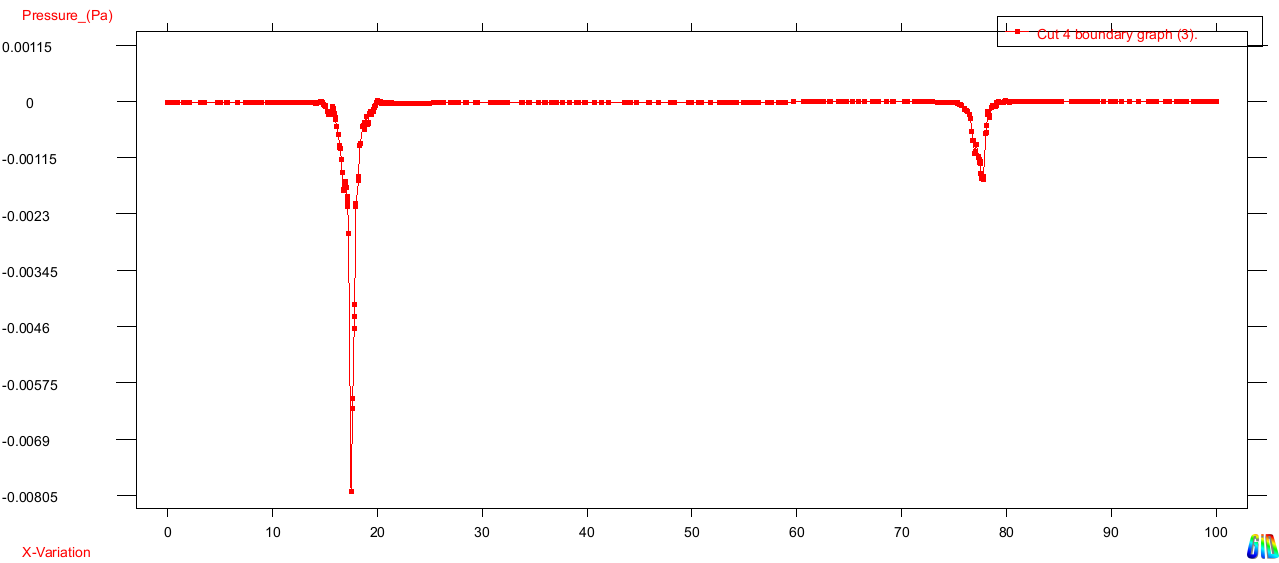
\includegraphics[scale=0.3]{img/100m/grf/100_grafico_presion_x_centro_pozos_distancia1}}
   \hspace{0.1\linewidth}
   %%----segunda subfigura----
   \subfloat[]{
        \label{100_grafico_velocidad_x_centro_pozos_distancia1}         %% Etiqueta para la segunda subfigura
        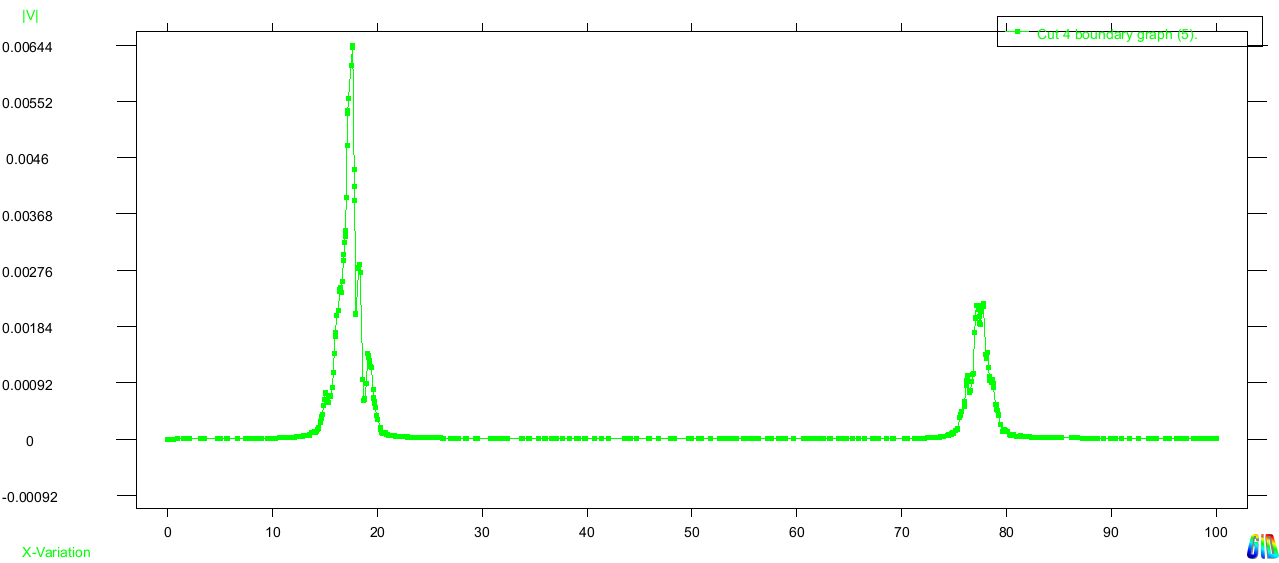
\includegraphics[scale=0.3]{img/100m/grf/100_grafico_velocidad_x_centro_pozos_distancia1}}
    \caption{Perfil de presión y velocidad para los pozos 1 y 2 de \emph{G1} situados a $1.0~[m]$ en dirección $-z$ de la base de los pozos. (\ref{100_grafico_presion_x_centro_pozos_distancia1}) Posición en $x$ vs. presión. - (\ref{100_grafico_velocidad_x_centro_pozos_distancia1}) Posición en $x$ vs. Módulo de Velocidad.}
   \label{100_grafico_velocidad_presion_centro_pozos_distancia1}                %% Etiqueta para la figura entera
\end{figure}

Se puede observar, que en las gráficas (\ref{100_grafico_velocidad_presion_centro_pozos_distancia0}), (\ref{100_grafico_velocidad_presion_centro_pozos_distancia05}) y (\ref{100_grafico_velocidad_presion_centro_pozos_distancia1}) a medida que se aleja de las bases de los pozos, el módulo de velocidad disminuye, mientras la presión aumenta. También, se puede ver, que existe una depresión mayor en el pozo 1 que en la base del pozo 2, conforme con las condiciones de bordes (velocidad en la base de los pozos) establecida en secciones anteriores.
%%%%%%%%%%%%%%%%%%%%%%%%%%%%%%%%%%%%%%%%%%%%%%%%%%%%%%%%%%
%%%%%%%%%%%%%%%%%%%%%%%%%%%%%%%%%%%%%%%%%%%%%%%%%%%%%%%%%%
%%%%%%%%%%%%%%%%%%%%%%%%%%%%%%%%%%%%%%%%%%%%%%%%%%%%%%%%%%
\subsection{Resultados para \emph{G2}}
%
\begin{figure}[tbhp]
\centerline{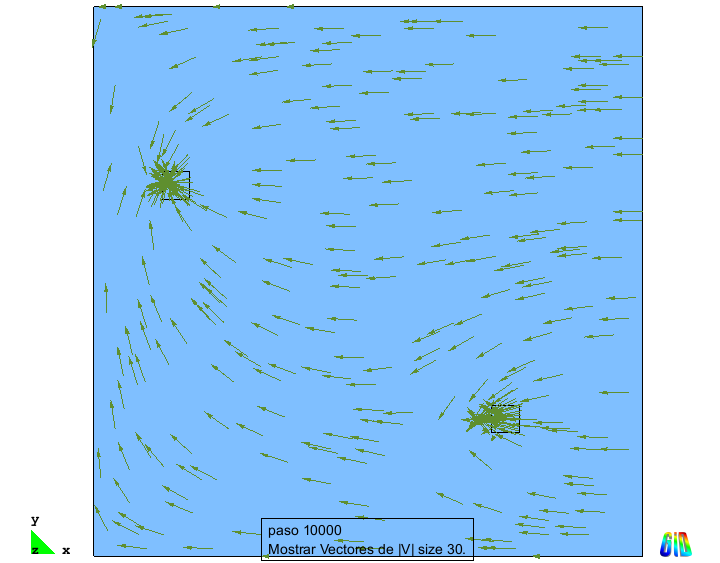
\includegraphics[scale=0.4]{img/200m/resul/200_xy_vectores}}
\caption{Vectores para \emph{G2}- Vista plano XY}
\label{200_xy_vectores}
\end{figure}
%
\begin{figure}[tbhp]
   \centering
   %%----primera subfigura----
   \subfloat[]{
        \label{200_XZ_presion_corte_centro_pozo1}         %% Etiqueta para la primera subfigura
        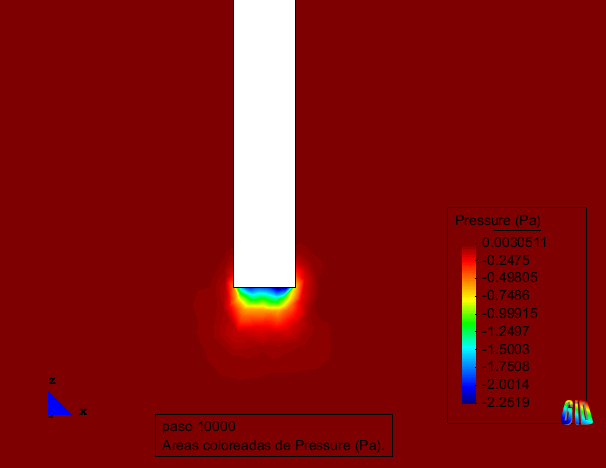
\includegraphics[scale=0.4]{img/200m/resul/200_XZ_presion_corte_centro_pozo1}}
   \hspace{0.1\linewidth}
   %%----segunda subfigura----
   \subfloat[]{
        \label{200_XZ_presion_corte_centro_pozo2}         %% Etiqueta para la segunda subfigura
        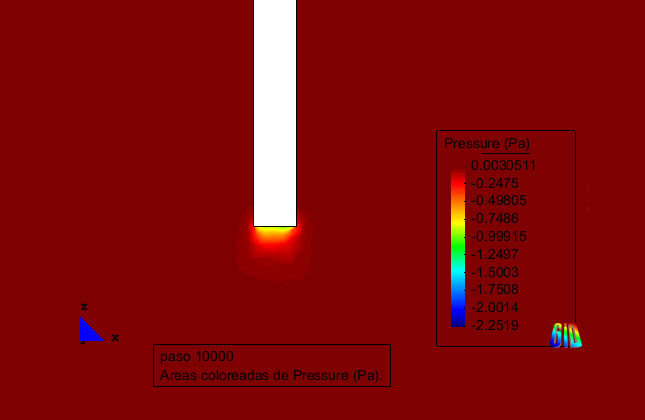
\includegraphics[scale=0.4]{img/200m/resul/200_XZ_presion_corte_centro_pozo2}}
    \caption{Corte a través del centro de ambos pozos para \emph{G2} - Vista en el plano XZ - (\ref{200_XZ_presion_corte_centro_pozo1}) Presión pozo 1. - (\ref{200_XZ_presion_corte_centro_pozo2})  Presión pozo 2.}
   \label{200_XZ_presion_corte_centro}                %% Etiqueta para la figura entera
\end{figure}
%
%
%corte centro pozos:
\begin{figure}[tbhp]
   \centering
   %%----primera subfigura----
   \subfloat[]{
        \label{200_XZ_velocidad_corte_centro_pozo1}         %% Etiqueta para la primera subfigura
        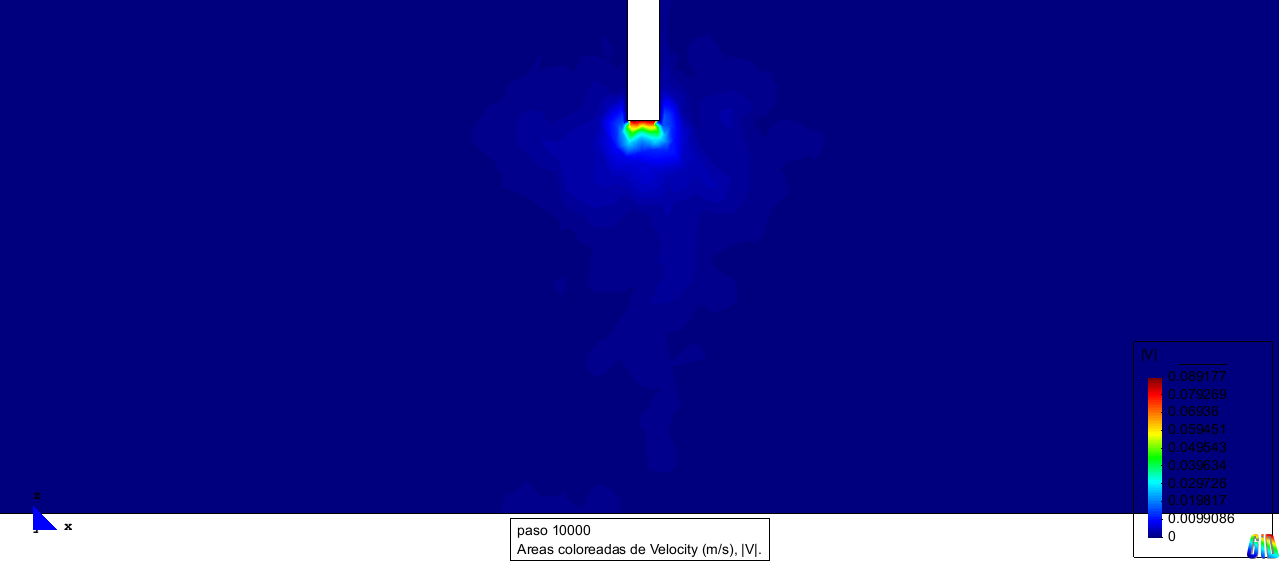
\includegraphics[scale=0.4]{img/200m/resul/200_XZ_velocidad_corte_centro_pozo1}}
   \hspace{0.1\linewidth}
   %%----segunda subfigura----
   \subfloat[]{
        \label{200_XZ_velocidad_corte_centro_pozo2}         %% Etiqueta para la segunda subfigura
        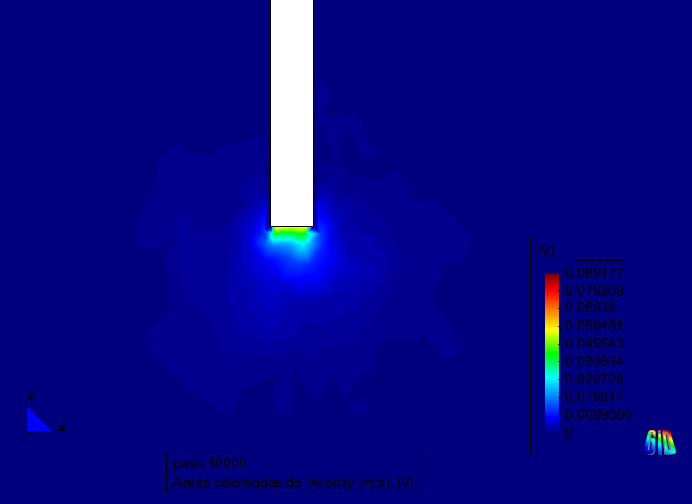
\includegraphics[scale=0.4]{img/200m/resul/200_XZ_velocidad_corte_centro_pozo2}}
    \caption{Corte a través del centro de ambos pozos para \emph{G2} -  - Vista en el plano XZ - (\ref{200_XZ_velocidad_corte_centro_pozo1}) Módulo de velocidad pozo 1. - (\ref{200_XZ_velocidad_corte_centro_pozo2}) Módulo de velocidad pozo 2.}
   \label{200_XZ_velocidad_corte_centro_pozos}                %% Etiqueta para la figura entera
\end{figure}
%
%
%corte horizontal:
\begin{figure}[tbhp]
   \centering
   %%----primera subfigura----
   \subfloat[]{
        \label{200_presion_horizontal}         %% Etiqueta para la primera subfigura
        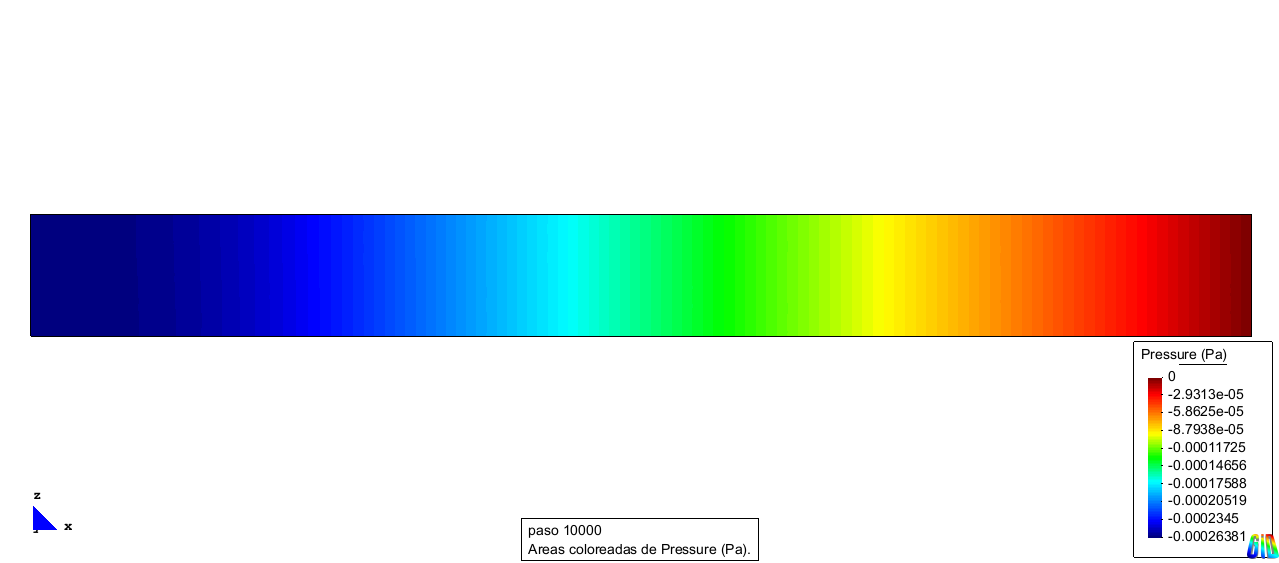
\includegraphics[scale=0.4]{img/200m/resul/200_XZ_presion_corte_horizontal}}
   \hspace{0.1\linewidth}
   %%----segunda subfigura----
   \subfloat[]{
        \label{200_velocidad_horizontal}         %% Etiqueta para la segunda subfigura
        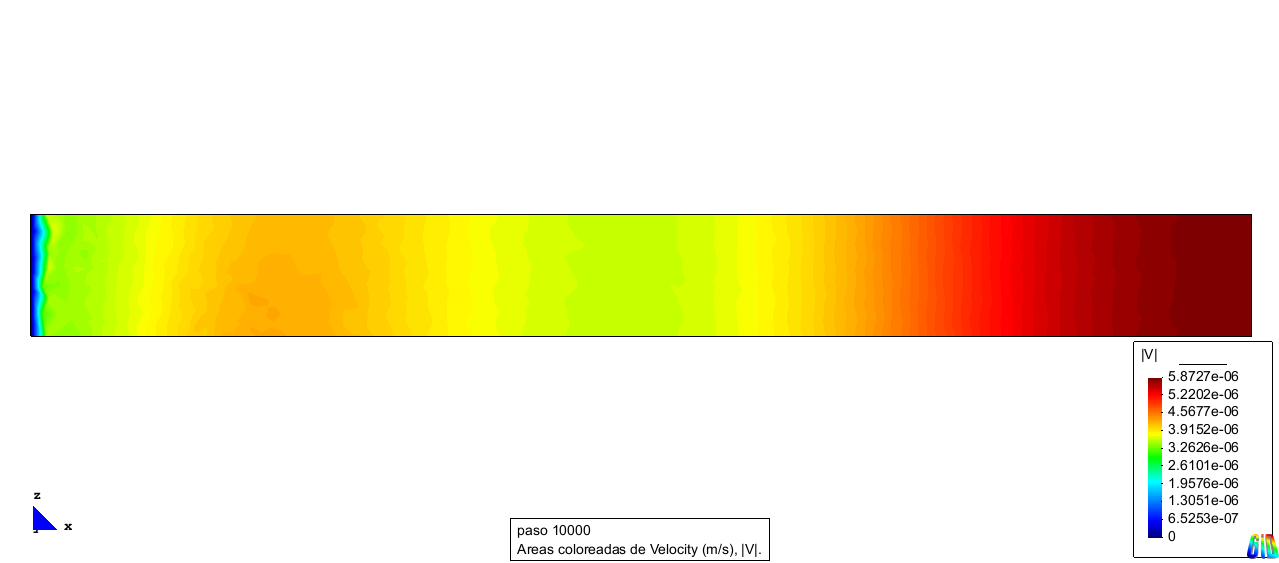
\includegraphics[scale=0.4]{img/200m/resul/200_XZ_velocidad_corte_horizontal}}
    \caption{Corte en $(x_1,y_1,z_1)=(0,50,0)$ hasta $(x_2,y_2,z_2)=(100,50,0)$ para \emph{G2} - Vista en el plano XZ - (\ref{200_presion_horizontal}) Presión. - (\ref{200_velocidad_horizontal}) Módulo de Velocidad.}
   \label{200_velocidad_presion_horizontal}                %% Etiqueta para la figura entera
\end{figure}
%
%
\begin{figure}[tbhp]
   \centering
   %%----primera subfigura----
   \subfloat[]{
        \label{200_presion_vertical}         %% Etiqueta para la primera subfigura
        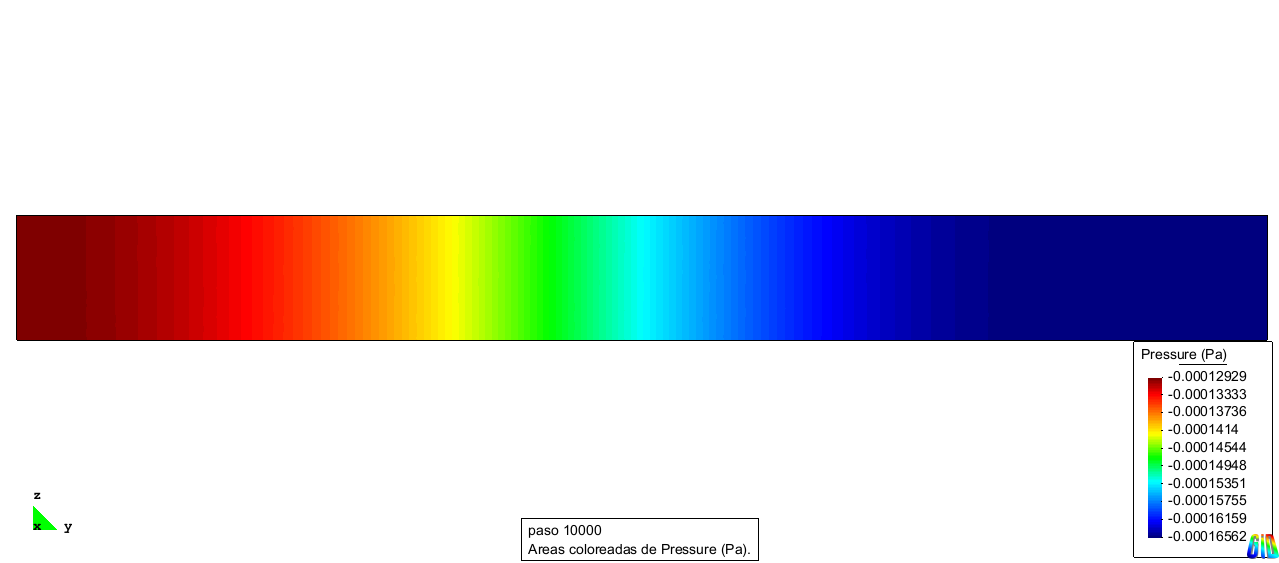
\includegraphics[scale=0.4]{img/200m/resul/200_ZY_presion_corte_vertical}}
   \hspace{0.1\linewidth}
   %%----segunda subfigura----
   \subfloat[]{
        \label{200_velocidad_vertical}         %% Etiqueta para la segunda subfigura
        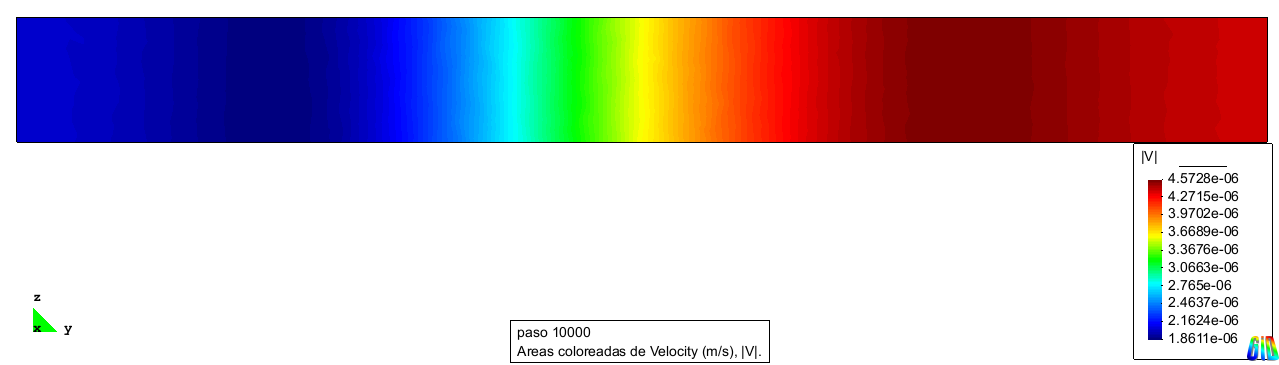
\includegraphics[scale=0.4]{img/200m/resul/200_ZY_velocidad_corte_vertical}}
    \caption{Corte en $(x_1,y_1,z_1)=(50,0,0)$ hasta $(x_2,y_2,z_2)=(50,100,0)$ para \emph{G2} - Vista en el plano YZ - (\ref{200_presion_vertical}) Presión. - (\ref{200_velocidad_vertical}) Módulo de Velocidad.}
   \label{200_velocidad_presion_vertical}                %% Etiqueta para la figura entera
\end{figure}
%%%%%%%%%%%%%%%%%%%%%%%%%%%%%%%%%%%%%%%%%%%%%%%%%%%%%%%%%%
%graficos00:
\begin{figure}[tbhp]
   \centering
   %%----primera subfigura----
   \subfloat[]{
        \label{200_grafico_presion_x_centro_pozos_distancia0}         %% Etiqueta para la primera subfigura
        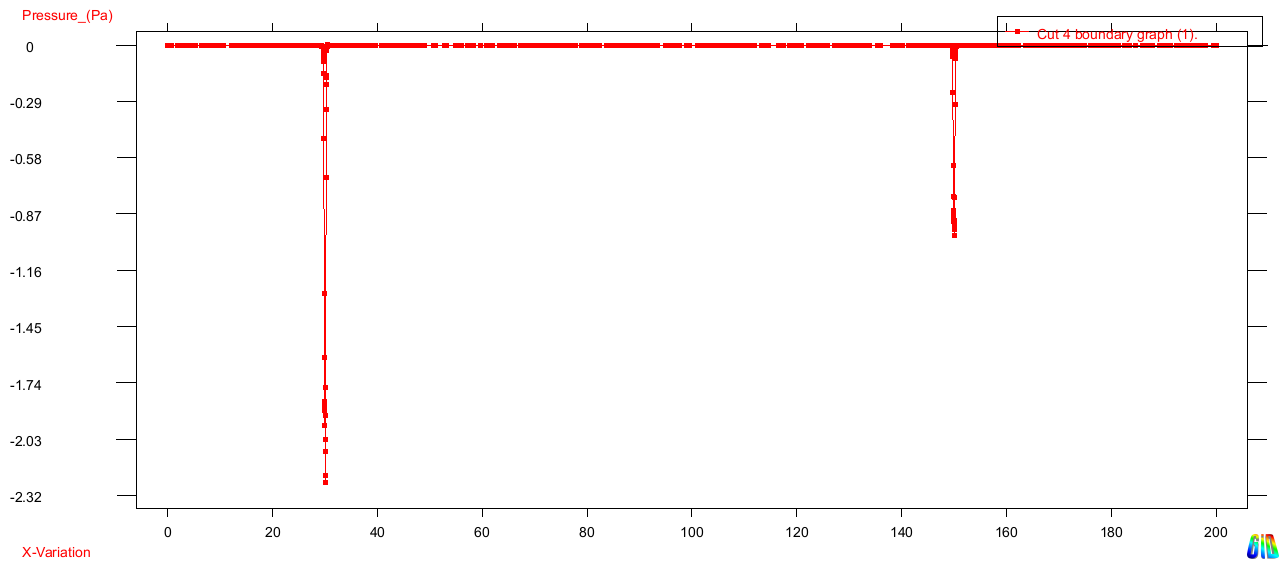
\includegraphics[scale=0.3]{img/200m/grf/200_grafico_presion_x_centro_pozos_distancia0}}
   \hspace{0.1\linewidth}
   %%----segunda subfigura----
   \subfloat[]{
        \label{200_grafico_velocidad_x_centro_pozos_distancia0}         %% Etiqueta para la segunda subfigura
        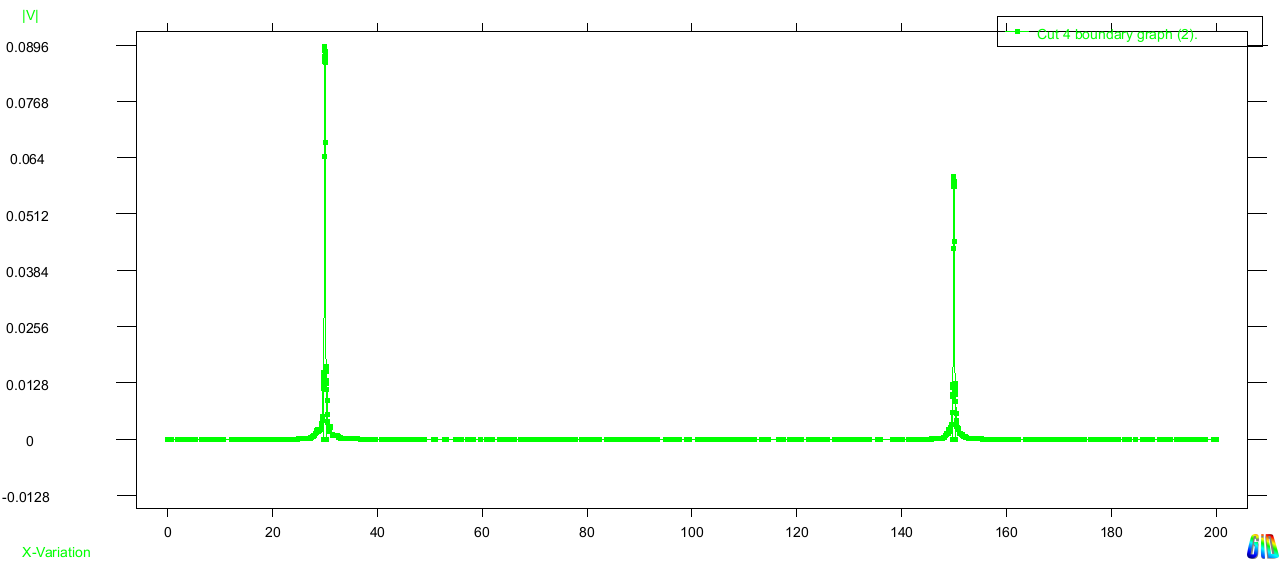
\includegraphics[scale=0.3]{img/200m/grf/200_grafico_velocidad_x_centro_pozos_distancia0}}
    \caption{Perfil de presión y velocidad para los pozos 1 y 2 de \emph{G2} situados sobre la base de los pozos. (\ref{200_grafico_presion_x_centro_pozos_distancia0}) Posición en $x$ vs. presión. - (\ref{200_grafico_velocidad_x_centro_pozos_distancia0}) Posición en $x$ vs. Módulo de Velocidad.}
   \label{200_grafico_velocidad_presion_centro_pozos_distancia0}                %% Etiqueta para la figura entera
\end{figure}
%
%graficos05:
\begin{figure}[tbhp]
   \centering
   %%----primera subfigura----
   \subfloat[]{
        \label{200_grafico_presion_x_centro_pozos_distancia05}         %% Etiqueta para la primera subfigura
        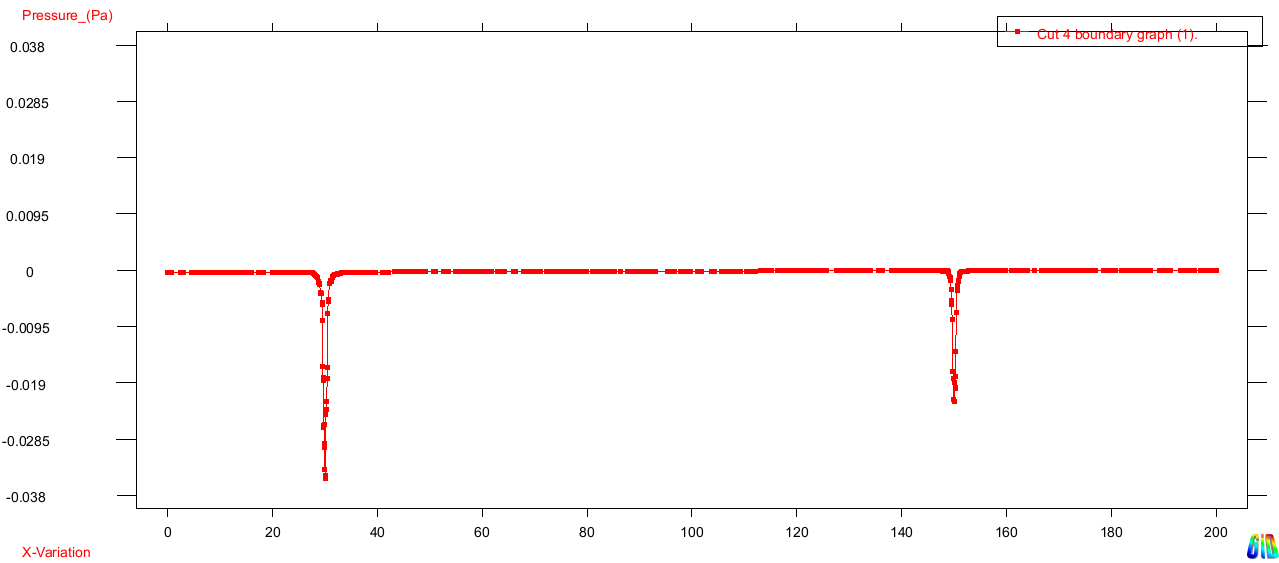
\includegraphics[scale=0.3]{img/200m/grf/200_grafico_presion_x_centro_pozos_distancia05}}
   \hspace{0.1\linewidth}
   %%----segunda subfigura----
   \subfloat[]{
        \label{200_grafico_velocidad_x_centro_pozos_distancia05}         %% Etiqueta para la segunda subfigura
        \includegraphics[scale=0.3]{img/200m/grf/200_grafico_velocidad_x_centro_pozos_distancia05}}
    \caption{Perfil de presión y velocidad para los pozos 1 y 2 de \emph{G2} situados a $0.5~[m]$ en dirección $-z$ de la base de los pozos. (\ref{200_grafico_presion_x_centro_pozos_distancia05}) Posición en $x$ vs. presión. - (\ref{200_grafico_velocidad_x_centro_pozos_distancia05}) Posición en $x$ vs. Módulo de Velocidad.}
   \label{200_grafico_velocidad_presion_centro_pozos_distancia05}                %% Etiqueta para la figura entera
\end{figure}
%graficos1:
\begin{figure}[tbhp]
   \centering
   %%----primera subfigura----
   \subfloat[]{
        \label{200_grafico_presion_x_centro_pozos_distancia1}         %% Etiqueta para la primera subfigura
        \includegraphics[scale=0.3]{img/200m/grf/200_grafico_presion_x_centro_pozos_distancia1}}
   \hspace{0.1\linewidth}
   %%----segunda subfigura----
   \subfloat[]{
        \label{200_grafico_velocidad_x_centro_pozos_distancia1}         %% Etiqueta para la segunda subfigura
        \includegraphics[scale=0.3]{img/200m/grf/200_grafico_velocidad_x_centro_pozos_distancia1}}
    \caption{Perfil de presión y velocidad para los pozos 1 y 2 de \emph{G2} situados a $1.0~[m]$ en dirección $-z$ de la base de los pozos. (\ref{200_grafico_presion_x_centro_pozos_distancia1}) Posición en $x$ vs. presión. - (\ref{200_grafico_velocidad_x_centro_pozos_distancia1}) Posición en $x$ vs. Módulo de Velocidad.}
   \label{200_grafico_velocidad_presion_centro_pozos_distancia1}                %% Etiqueta para la figura entera
\end{figure}
%v(veloc) -> lineas de flujo/vect
%p->equipotenciales
%realizar cortes
%lo que vamos a ver va a ser las equipotenciales (lineas de presion que son perpendiculares al flujo).siempre es contraria a la linea de velocidad\\
%En los softwares específicos de hidrogeología, fijate que aca tenes el esquema de calculo que es una malla muy guresa en dos dimensiones, que te va a dar isocurvas de niveles. Se va a ver como esto va bombeando y ese nivel de agua cerca de la bomba va ir deprimiendose formando el cono de desenso. Eso, asi de esa forma aca no lo vamos a poder hacer, porque para poder hacer eso en 3D (en 2D si se puede) tenes que tener un soft que distinga entre suelo no saturado y suelo saturado. En el suelo saturado las ecs de gobierno son distintas a las del no saturado. El soft que tenemos solamente tiene las ecs de gob del suelo saturado, el no saturado tiene un modelo mucho mas complejo, en realidad estos modelos son bidimensionales porque no calculan el flujo en suelo saturado, lo que calculan seria la curva, la interfaz, seria la sup que los separa, nada mas, sería la ubicación de esa sup que distingue zona saturada de la no saturada. que tiene ecuaciones simples, pero no calcula detalles del flujo, este modelo calcula el flujo en suelo saturado. 
%Se coincidiera que se esta en presencia de un estrato de suleo saturado (esto es saturado de agua). 
%Vamos a tener lineas equipotenciales (unen lineas de igual potencial hidráulico) las cuales son perpendiculares a las lineas del flujo y serian valores de presión que ejerce el agua sobre el suelo. Esas líneas equipotenciales van a ser equivalentes en interpretación a las lineas de superficie que se calculan tradicionalmente en hidrologia.
%%%%%%%%%%%%%%%%%%%%%%%%%%%%%%%%%%%%%%%%%%%%%%%%%%%%%%%%%%%%%%%%%%%%%%%%%%%%%%%%%%%%%%%%%%%%%%%%%%
%%%%%%%%%%%%%%%%%%%%%%%%%%%%%%%%%%%%%%%%%%%%%%%%%%%%%%%%%%%%%%%%%%%%%%%%%%%%%%%%%%%%%%%%%%%%%%%%%%
%%%%%%%%%%%%%%%%%%%%%%%%%%%%%%%%%%%%%%%%%%%%%%%%%%%%%%%%%%%%%%%%%%%%%%%%%%%%%%%%%%%%%%%%%%%%%%%%%%
\section{Conclusiones}
%si el mod respondio
%que problemas tuvimos? ahi hacer mencion al pozo grande y tiempo de calculo...
%pozo real vs pozo simulado
%%%%%%%%%%%%%%%%%%%%%%%%%%%%%%%%%%%%%%%%%%%%%%%%%
%%%%%%%%%%%%%%%%%%%%%%%%%%%%%%%%%%%%%%%%%%%%%%%%%
%%%%%%%%%%%%%%%%%%%%%%%%%%%%%%%%%%%%%%%%%%%%%%%%%
\end{document}